\documentclass[a4paper,titlepage,11pt,twosides,floatssmall]{mwrep}
\usepackage[left=2.5cm,right=2.5cm,top=2.5cm,bottom=2.5cm]{geometry}
\usepackage[OT1]{fontenc}
\usepackage{polski}
\usepackage{amsmath}
\usepackage{amsfonts}
\usepackage{amssymb}
\usepackage{graphicx}
\usepackage{url}
\usepackage{tikz}
\usetikzlibrary{arrows,calc,decorations.markings,math,arrows.meta}
\usepackage{rotating}
\usepackage[percent]{overpic}
\usepackage[cp1250]{inputenc}
\usepackage{xcolor}
\usepackage{pgfplots}
\usetikzlibrary{pgfplots.groupplots}
\usepackage{listings}
\usepackage{matlab-prettifier}
\usepackage{enumitem,amssymb}
\definecolor{szary}{rgb}{0.95,0.95,0.95}
\usepackage{siunitx}
\sisetup{detect-weight,exponent-product=\cdot,output-decimal-marker={,},per-mode=symbol,binary-units=true,range-phrase={-},range-units=single}
\SendSettingsToPgf
%konfiguracje pakietu listings
\lstset{
	backgroundcolor=\color{szary},
	frame=single,
	breaklines=true,
}
\lstdefinestyle{customlatex}{
	basicstyle=\footnotesize\ttfamily,
	%basicstyle=\small\ttfamily,
}
\lstdefinestyle{customc}{
	breaklines=true,
	frame=tb,
	language=C,
	xleftmargin=0pt,
	showstringspaces=false,
	basicstyle=\small\ttfamily,
	keywordstyle=\bfseries\color{green!40!black},
	commentstyle=\itshape\color{purple!40!black},
	identifierstyle=\color{blue},
	stringstyle=\color{orange},
}
\lstdefinestyle{custommatlab}{
	captionpos=t,
	breaklines=true,
	frame=tb,
	xleftmargin=0pt,
	language=matlab,
	showstringspaces=false,
	%basicstyle=\footnotesize\ttfamily,
	basicstyle=\scriptsize\ttfamily,
	keywordstyle=\bfseries\color{green!40!black},
	commentstyle=\itshape\color{purple!40!black},
	identifierstyle=\color{blue},
	stringstyle=\color{orange},
}

%wymiar tekstu (bez �ywej paginy)
\textwidth 160mm \textheight 247mm

%ustawienia pakietu pgfplots
\pgfplotsset{
tick label style={font=\scriptsize},
label style={font=\small},
legend style={font=\small},
title style={font=\small}
}

\def\figurename{Rys.}
\def\tablename{Tab.}

%konfiguracja liczby p�ywaj�cych element�w
\setcounter{topnumber}{0}%2
\setcounter{bottomnumber}{3}%1
\setcounter{totalnumber}{5}%3
\renewcommand{\textfraction}{0.01}%0.2
\renewcommand{\topfraction}{0.95}%0.7
\renewcommand{\bottomfraction}{0.95}%0.3
\renewcommand{\floatpagefraction}{0.35}%0.5

\begin{document}
\frenchspacing
\pagestyle{uheadings}

%strona tytu�owa
\title{\bf Sprawozdanie z projektu nr 4, zadanie nr 3\vskip 0.1cm}
\author{Jakub Gruszecki, Wojciech Rokicki, Rados�aw Pietkun}
\date{2020}

\makeatletter
\renewcommand{\maketitle}{\begin{titlepage}
\begin{center}{\LARGE {\bf
Wydzia� Elektroniki i Technik Informacyjnych}}\\
\vspace{0.4cm}
{\LARGE {\bf Politechnika Warszawska}}\\
\vspace{0.3cm}
\end{center}
\vspace{5cm}
\begin{center}
{\bf \LARGE Projektowanie uk�ad�w sterowania\\ (projekt grupowy) \vskip 0.1cm}
\end{center}
\vspace{1cm}
\begin{center}
{\bf \LARGE \@title}
\end{center}
\vspace{2cm}
\begin{center}
{\bf \Large \@author \par}
\end{center}
\vspace*{\stretch{6}}
\begin{center}
\bf{\large{Warszawa, \@date\vskip 0.1cm}}
\end{center}
\end{titlepage}
}
\makeatother

\maketitle

\tableofcontents
\chapter{Sprawdzenie poprawno�ci punktu pracy}

\section{Poprawno�� warto�ci sygna��w w punkcie pracy}
W celu sprawdzenia poprawno�ci warto�ci sygna��w $U_{\mathrm{pp}}$ oraz $Y_{\mathrm{pp}}$ obiekt zosta� pobudzony sygna�em o warto�ci: $U_{\mathrm{pp}}=\num{0}$. Warto�ci sygna��w w punkcie pracy b�d� poprawne, je�li sygna� wyj�ciowy przyjmie warto�� sta�� $Y_{\mathrm{pp}}=\num{0}$.

\begin{figure}[h!]
\centering
% This file was created by matlab2tikz.
%
\definecolor{mycolor1}{rgb}{0.00000,0.44700,0.74100}%
%
\begin{tikzpicture}

\begin{axis}[%
width=4.521in,
height=1.493in,
at={(0.758in,2.554in)},
scale only axis,
xmin=0,
xmax=400,
ymin=-1,
ymax=1,
axis background/.style={fill=white},
title style={font=\bfseries},
title={U},
legend style={legend cell align=left, align=left, draw=white!15!black}
]
\addplot [color=mycolor1]
  table[row sep=crcr]{%
1	0\\
2	0\\
3	0\\
4	0\\
5	0\\
6	0\\
7	0\\
8	0\\
9	0\\
10	0\\
11	0\\
12	0\\
13	0\\
14	0\\
15	0\\
16	0\\
17	0\\
18	0\\
19	0\\
20	0\\
21	0\\
22	0\\
23	0\\
24	0\\
25	0\\
26	0\\
27	0\\
28	0\\
29	0\\
30	0\\
31	0\\
32	0\\
33	0\\
34	0\\
35	0\\
36	0\\
37	0\\
38	0\\
39	0\\
40	0\\
41	0\\
42	0\\
43	0\\
44	0\\
45	0\\
46	0\\
47	0\\
48	0\\
49	0\\
50	0\\
51	0\\
52	0\\
53	0\\
54	0\\
55	0\\
56	0\\
57	0\\
58	0\\
59	0\\
60	0\\
61	0\\
62	0\\
63	0\\
64	0\\
65	0\\
66	0\\
67	0\\
68	0\\
69	0\\
70	0\\
71	0\\
72	0\\
73	0\\
74	0\\
75	0\\
76	0\\
77	0\\
78	0\\
79	0\\
80	0\\
81	0\\
82	0\\
83	0\\
84	0\\
85	0\\
86	0\\
87	0\\
88	0\\
89	0\\
90	0\\
91	0\\
92	0\\
93	0\\
94	0\\
95	0\\
96	0\\
97	0\\
98	0\\
99	0\\
100	0\\
101	0\\
102	0\\
103	0\\
104	0\\
105	0\\
106	0\\
107	0\\
108	0\\
109	0\\
110	0\\
111	0\\
112	0\\
113	0\\
114	0\\
115	0\\
116	0\\
117	0\\
118	0\\
119	0\\
120	0\\
121	0\\
122	0\\
123	0\\
124	0\\
125	0\\
126	0\\
127	0\\
128	0\\
129	0\\
130	0\\
131	0\\
132	0\\
133	0\\
134	0\\
135	0\\
136	0\\
137	0\\
138	0\\
139	0\\
140	0\\
141	0\\
142	0\\
143	0\\
144	0\\
145	0\\
146	0\\
147	0\\
148	0\\
149	0\\
150	0\\
151	0\\
152	0\\
153	0\\
154	0\\
155	0\\
156	0\\
157	0\\
158	0\\
159	0\\
160	0\\
161	0\\
162	0\\
163	0\\
164	0\\
165	0\\
166	0\\
167	0\\
168	0\\
169	0\\
170	0\\
171	0\\
172	0\\
173	0\\
174	0\\
175	0\\
176	0\\
177	0\\
178	0\\
179	0\\
180	0\\
181	0\\
182	0\\
183	0\\
184	0\\
185	0\\
186	0\\
187	0\\
188	0\\
189	0\\
190	0\\
191	0\\
192	0\\
193	0\\
194	0\\
195	0\\
196	0\\
197	0\\
198	0\\
199	0\\
200	0\\
201	0\\
202	0\\
203	0\\
204	0\\
205	0\\
206	0\\
207	0\\
208	0\\
209	0\\
210	0\\
211	0\\
212	0\\
213	0\\
214	0\\
215	0\\
216	0\\
217	0\\
218	0\\
219	0\\
220	0\\
221	0\\
222	0\\
223	0\\
224	0\\
225	0\\
226	0\\
227	0\\
228	0\\
229	0\\
230	0\\
231	0\\
232	0\\
233	0\\
234	0\\
235	0\\
236	0\\
237	0\\
238	0\\
239	0\\
240	0\\
241	0\\
242	0\\
243	0\\
244	0\\
245	0\\
246	0\\
247	0\\
248	0\\
249	0\\
250	0\\
251	0\\
252	0\\
253	0\\
254	0\\
255	0\\
256	0\\
257	0\\
258	0\\
259	0\\
260	0\\
261	0\\
262	0\\
263	0\\
264	0\\
265	0\\
266	0\\
267	0\\
268	0\\
269	0\\
270	0\\
271	0\\
272	0\\
273	0\\
274	0\\
275	0\\
276	0\\
277	0\\
278	0\\
279	0\\
280	0\\
281	0\\
282	0\\
283	0\\
284	0\\
285	0\\
286	0\\
287	0\\
288	0\\
289	0\\
290	0\\
291	0\\
292	0\\
293	0\\
294	0\\
295	0\\
296	0\\
297	0\\
298	0\\
299	0\\
300	0\\
301	0\\
302	0\\
303	0\\
304	0\\
305	0\\
306	0\\
307	0\\
308	0\\
309	0\\
310	0\\
311	0\\
312	0\\
313	0\\
314	0\\
315	0\\
316	0\\
317	0\\
318	0\\
319	0\\
320	0\\
321	0\\
322	0\\
323	0\\
324	0\\
325	0\\
326	0\\
327	0\\
328	0\\
329	0\\
330	0\\
331	0\\
332	0\\
333	0\\
334	0\\
335	0\\
336	0\\
337	0\\
338	0\\
339	0\\
340	0\\
341	0\\
342	0\\
343	0\\
344	0\\
345	0\\
346	0\\
347	0\\
348	0\\
349	0\\
350	0\\
351	0\\
352	0\\
353	0\\
354	0\\
355	0\\
356	0\\
357	0\\
358	0\\
359	0\\
360	0\\
361	0\\
362	0\\
363	0\\
364	0\\
365	0\\
366	0\\
367	0\\
368	0\\
369	0\\
370	0\\
371	0\\
372	0\\
373	0\\
374	0\\
375	0\\
376	0\\
377	0\\
378	0\\
379	0\\
380	0\\
381	0\\
382	0\\
383	0\\
384	0\\
385	0\\
386	0\\
387	0\\
388	0\\
389	0\\
390	0\\
391	0\\
392	0\\
393	0\\
394	0\\
395	0\\
396	0\\
397	0\\
398	0\\
399	0\\
400	0\\
};

\end{axis}

\begin{axis}[%
width=4.521in,
height=1.493in,
at={(0.758in,0.481in)},
scale only axis,
xmin=0,
xmax=400,
ymin=-1,
ymax=1,
axis background/.style={fill=white},
title style={font=\bfseries},
title={Y},
legend style={legend cell align=left, align=left, draw=white!15!black}
]
\addplot [color=mycolor1]
  table[row sep=crcr]{%
1	0\\
2	0\\
3	0\\
4	0\\
5	0\\
6	0\\
7	0\\
8	0\\
9	0\\
10	0\\
11	0\\
12	0\\
13	0\\
14	0\\
15	0\\
16	0\\
17	0\\
18	0\\
19	0\\
20	0\\
21	0\\
22	0\\
23	0\\
24	0\\
25	0\\
26	0\\
27	0\\
28	0\\
29	0\\
30	0\\
31	0\\
32	0\\
33	0\\
34	0\\
35	0\\
36	0\\
37	0\\
38	0\\
39	0\\
40	0\\
41	0\\
42	0\\
43	0\\
44	0\\
45	0\\
46	0\\
47	0\\
48	0\\
49	0\\
50	0\\
51	0\\
52	0\\
53	0\\
54	0\\
55	0\\
56	0\\
57	0\\
58	0\\
59	0\\
60	0\\
61	0\\
62	0\\
63	0\\
64	0\\
65	0\\
66	0\\
67	0\\
68	0\\
69	0\\
70	0\\
71	0\\
72	0\\
73	0\\
74	0\\
75	0\\
76	0\\
77	0\\
78	0\\
79	0\\
80	0\\
81	0\\
82	0\\
83	0\\
84	0\\
85	0\\
86	0\\
87	0\\
88	0\\
89	0\\
90	0\\
91	0\\
92	0\\
93	0\\
94	0\\
95	0\\
96	0\\
97	0\\
98	0\\
99	0\\
100	0\\
101	0\\
102	0\\
103	0\\
104	0\\
105	0\\
106	0\\
107	0\\
108	0\\
109	0\\
110	0\\
111	0\\
112	0\\
113	0\\
114	0\\
115	0\\
116	0\\
117	0\\
118	0\\
119	0\\
120	0\\
121	0\\
122	0\\
123	0\\
124	0\\
125	0\\
126	0\\
127	0\\
128	0\\
129	0\\
130	0\\
131	0\\
132	0\\
133	0\\
134	0\\
135	0\\
136	0\\
137	0\\
138	0\\
139	0\\
140	0\\
141	0\\
142	0\\
143	0\\
144	0\\
145	0\\
146	0\\
147	0\\
148	0\\
149	0\\
150	0\\
151	0\\
152	0\\
153	0\\
154	0\\
155	0\\
156	0\\
157	0\\
158	0\\
159	0\\
160	0\\
161	0\\
162	0\\
163	0\\
164	0\\
165	0\\
166	0\\
167	0\\
168	0\\
169	0\\
170	0\\
171	0\\
172	0\\
173	0\\
174	0\\
175	0\\
176	0\\
177	0\\
178	0\\
179	0\\
180	0\\
181	0\\
182	0\\
183	0\\
184	0\\
185	0\\
186	0\\
187	0\\
188	0\\
189	0\\
190	0\\
191	0\\
192	0\\
193	0\\
194	0\\
195	0\\
196	0\\
197	0\\
198	0\\
199	0\\
200	0\\
201	0\\
202	0\\
203	0\\
204	0\\
205	0\\
206	0\\
207	0\\
208	0\\
209	0\\
210	0\\
211	0\\
212	0\\
213	0\\
214	0\\
215	0\\
216	0\\
217	0\\
218	0\\
219	0\\
220	0\\
221	0\\
222	0\\
223	0\\
224	0\\
225	0\\
226	0\\
227	0\\
228	0\\
229	0\\
230	0\\
231	0\\
232	0\\
233	0\\
234	0\\
235	0\\
236	0\\
237	0\\
238	0\\
239	0\\
240	0\\
241	0\\
242	0\\
243	0\\
244	0\\
245	0\\
246	0\\
247	0\\
248	0\\
249	0\\
250	0\\
251	0\\
252	0\\
253	0\\
254	0\\
255	0\\
256	0\\
257	0\\
258	0\\
259	0\\
260	0\\
261	0\\
262	0\\
263	0\\
264	0\\
265	0\\
266	0\\
267	0\\
268	0\\
269	0\\
270	0\\
271	0\\
272	0\\
273	0\\
274	0\\
275	0\\
276	0\\
277	0\\
278	0\\
279	0\\
280	0\\
281	0\\
282	0\\
283	0\\
284	0\\
285	0\\
286	0\\
287	0\\
288	0\\
289	0\\
290	0\\
291	0\\
292	0\\
293	0\\
294	0\\
295	0\\
296	0\\
297	0\\
298	0\\
299	0\\
300	0\\
301	0\\
302	0\\
303	0\\
304	0\\
305	0\\
306	0\\
307	0\\
308	0\\
309	0\\
310	0\\
311	0\\
312	0\\
313	0\\
314	0\\
315	0\\
316	0\\
317	0\\
318	0\\
319	0\\
320	0\\
321	0\\
322	0\\
323	0\\
324	0\\
325	0\\
326	0\\
327	0\\
328	0\\
329	0\\
330	0\\
331	0\\
332	0\\
333	0\\
334	0\\
335	0\\
336	0\\
337	0\\
338	0\\
339	0\\
340	0\\
341	0\\
342	0\\
343	0\\
344	0\\
345	0\\
346	0\\
347	0\\
348	0\\
349	0\\
350	0\\
351	0\\
352	0\\
353	0\\
354	0\\
355	0\\
356	0\\
357	0\\
358	0\\
359	0\\
360	0\\
361	0\\
362	0\\
363	0\\
364	0\\
365	0\\
366	0\\
367	0\\
368	0\\
369	0\\
370	0\\
371	0\\
372	0\\
373	0\\
374	0\\
375	0\\
376	0\\
377	0\\
378	0\\
379	0\\
380	0\\
381	0\\
382	0\\
383	0\\
384	0\\
385	0\\
386	0\\
387	0\\
388	0\\
389	0\\
390	0\\
391	0\\
392	0\\
393	0\\
394	0\\
395	0\\
396	0\\
397	0\\
398	0\\
399	0\\
400	0\\
};

\end{axis}

\begin{axis}[%
width=5.833in,
height=4.375in,
at={(0in,0in)},
scale only axis,
xmin=0,
xmax=1,
ymin=0,
ymax=1,
axis line style={draw=none},
ticks=none,
axis x line*=bottom,
axis y line*=left,
legend style={legend cell align=left, align=left, draw=white!15!black}
]
\end{axis}
\end{tikzpicture}%
\caption{Przebiegi sygna��w u(k), y(k) w punkcie pracy}
\label{punkt_pracy}
\end{figure}

\section{Wnioski}
Na podstawie rysunku \ref{punkt_pracy} wida�, �e dla sta�ej warto�ci sygna�u steruj�cego $U_{\mathrm{pp}}=\num{0}$ wyj�cie obiektu przyjmuje sta�� warto��, r�wn� $Y_{\mathrm{pp}}=~\num{0}$. Jest to dow�d na to, �e podane warto�ci sygna��w wej�ciowego sterowania oraz wyj�ciowego w punkcie pracy s� poprawne.

\section{Implementacja}
Do przeprowadzenia eksperymentu wykorzystany zosta� skrypt \verb+zad1.m+.
\chapter{Odpowiedzi skokowe i charakterystyka statyczna}

\section{Wyznaczenie dpowiedzi skokowych}
W celu wyznaczenia odpowiedzi skokowych obiekt pobudzony zosta� czterema skokami sygna�u steruj�cego w chwili k=21. Sygna� steruj�cy zmienia� si� o $dU$=0,1 od $U_{min}$=0,9 do $U_{max}$=1,3.

\begin{figure}[h!]
\centering
% This file was created by matlab2tikz.
%
%The latest updates can be retrieved from
%  http://www.mathworks.com/matlabcentral/fileexchange/22022-matlab2tikz-matlab2tikz
%where you can also make suggestions and rate matlab2tikz.
%
\definecolor{mycolor1}{rgb}{0.00000,0.44700,0.74100}%
\definecolor{mycolor2}{rgb}{0.85000,0.32500,0.09800}%
\definecolor{mycolor3}{rgb}{0.92900,0.69400,0.12500}%
\definecolor{mycolor4}{rgb}{0.49400,0.18400,0.55600}%
%
\begin{tikzpicture}

\begin{axis}[%
width=4.521in,
height=1.488in,
at={(0.758in,2.554in)},
scale only axis,
xmin=0,
xmax=600,
ymin=1.36443365695792,
ymax=2.63556634304209,
axis background/.style={fill=white},
title style={font=\bfseries},
title={Sygnal wyjsciowy},
legend style={legend cell align=left, align=left, draw=white!15!black}
]
\addplot [color=mycolor1]
  table[row sep=crcr]{%
1	2\\
2	2\\
3	2\\
4	2\\
5	2\\
6	2\\
7	2\\
8	2\\
9	2\\
10	2\\
11	2\\
12	2\\
13	2\\
14	2\\
15	2\\
16	2\\
17	2\\
18	2\\
19	2\\
20	2\\
21	2\\
22	2\\
23	2\\
24	2\\
25	2\\
26	2\\
27	2\\
28	2\\
29	2\\
30	2\\
31	1.9979816\\
32	1.99235773848\\
33	1.98371668135674\\
34	1.97257503023226\\
35	1.95938553170158\\
36	1.94454408239941\\
37	1.92839600996488\\
38	1.91124170226892\\
39	1.89334165017042\\
40	1.87492096267203\\
41	1.85617340756908\\
42	1.83726502546675\\
43	1.81833736032739\\
44	1.79951034545341\\
45	1.78088487996797\\
46	1.76254512738566\\
47	1.74456056473254\\
48	1.72698780784788\\
49	1.70987223594765\\
50	1.69324943622739\\
51	1.6771464872043\\
52	1.66158309762431\\
53	1.64657261606932\\
54	1.63212292487534\\
55	1.61823723059774\\
56	1.60491476202054\\
57	1.59215138559002\\
58	1.57994014714617\\
59	1.56827174791886\\
60	1.55713496193878\\
61	1.54651700127759\\
62	1.53640383486921\\
63	1.52678046606834\\
64	1.51763117356549\\
65	1.50893971979504\\
66	1.50068953053909\\
67	1.49286384903899\\
68	1.48544586757572\\
69	1.47841883916507\\
70	1.47176617172999\\
71	1.46547150685825\\
72	1.45951878502523\\
73	1.45389229895657\\
74	1.44857673662161\\
75	1.44355721518399\\
76	1.43881930708764\\
77	1.43434905932444\\
78	1.43013300681122\\
79	1.42615818069774\\
80	1.42241211233249\\
81	1.41888283352845\\
82	1.41555887369521\\
83	1.41242925433613\\
84	1.40948348134926\\
85	1.40671153551659\\
86	1.40410386151866\\
87	1.40165135576871\\
88	1.39934535332284\\
89	1.39717761408892\\
90	1.39514030852713\\
91	1.39322600300849\\
92	1.39142764497447\\
93	1.3897385480199\\
94	1.38815237700302\\
95	1.38666313327078\\
96	1.3852651400727\\
97	1.38395302822474\\
98	1.38272172207325\\
99	1.38156642579973\\
100	1.38048261009867\\
101	1.37946599925363\\
102	1.37851255863013\\
103	1.37761848259882\\
104	1.37678018289737\\
105	1.37599427743579\\
106	1.37525757954611\\
107	1.37456708767486\\
108	1.37391997551386\\
109	1.37331358256314\\
110	1.37274540511797\\
111	1.37221308767055\\
112	1.37171441471586\\
113	1.37124730295023\\
114	1.37080979385063\\
115	1.370400046622\\
116	1.37001633149978\\
117	1.36965702339446\\
118	1.36932059586489\\
119	1.36900561540721\\
120	1.36871073604618\\
121	1.36843469421589\\
122	1.36817630391714\\
123	1.36793445213884\\
124	1.36770809453132\\
125	1.36749625131951\\
126	1.36729800344442\\
127	1.36711248892183\\
128	1.36693889940721\\
129	1.36677647695653\\
130	1.3666245109729\\
131	1.36648233532925\\
132	1.36634932565809\\
133	1.36622489679907\\
134	1.36610850039628\\
135	1.36599962263679\\
136	1.36589778212304\\
137	1.36580252787144\\
138	1.36571343743031\\
139	1.36563011511037\\
140	1.36555219032161\\
141	1.36547931601024\\
142	1.3654111671902\\
143	1.36534743956378\\
144	1.36528784822606\\
145	1.36523212644847\\
146	1.36518002453673\\
147	1.36513130875884\\
148	1.36508576033904\\
149	1.36504317451375\\
150	1.36500335964587\\
151	1.36496613639389\\
152	1.36493133693264\\
153	1.36489880422244\\
154	1.36486839132382\\
155	1.36483996075501\\
156	1.36481338388965\\
157	1.36478854039223\\
158	1.36476531768891\\
159	1.36474361047169\\
160	1.36472332023373\\
161	1.36470435483407\\
162	1.36468662808968\\
163	1.3646700593935\\
164	1.36465457335651\\
165	1.36464009947257\\
166	1.36462657180455\\
167	1.36461392869038\\
168	1.36460211246778\\
169	1.36459106921663\\
170	1.36458074851764\\
171	1.36457110322652\\
172	1.36456208926255\\
173	1.36455366541068\\
174	1.36454579313632\\
175	1.36453843641193\\
176	1.36453156155485\\
177	1.36452513707541\\
178	1.36451913353494\\
179	1.36451352341275\\
180	1.36450828098183\\
181	1.36450338219243\\
182	1.36449880456324\\
183	1.36449452707947\\
184	1.36449053009767\\
185	1.3644867952565\\
186	1.36448330539347\\
187	1.36448004446688\\
188	1.36447699748293\\
189	1.36447415042752\\
190	1.36447149020241\\
191	1.3644690045656\\
192	1.36446668207555\\
193	1.36446451203894\\
194	1.36446248446195\\
195	1.3644605900046\\
196	1.36445881993812\\
197	1.36445716610503\\
198	1.36445562088186\\
199	1.3644541771443\\
200	1.36445282823459\\
201	1.364451567931\\
202	1.3644503904194\\
203	1.3644492902666\\
204	1.3644482623954\\
205	1.36444730206139\\
206	1.36444640483111\\
207	1.36444556656177\\
208	1.36444478338219\\
209	1.36444405167504\\
210	1.36444336806021\\
211	1.36444272937932\\
212	1.36444213268116\\
213	1.36444157520813\\
214	1.36444105438357\\
215	1.36444056779991\\
216	1.36444011320757\\
217	1.36443968850462\\
218	1.36443929172711\\
219	1.36443892104001\\
220	1.36443857472877\\
221	1.3644382511914\\
222	1.36443794893113\\
223	1.36443766654946\\
224	1.36443740273975\\
225	1.36443715628117\\
226	1.3644369260331\\
227	1.36443671092982\\
228	1.36443650997566\\
229	1.36443632224033\\
230	1.36443614685468\\
231	1.36443598300667\\
232	1.36443582993763\\
233	1.36443568693873\\
234	1.36443555334775\\
235	1.36443542854596\\
236	1.36443531195533\\
237	1.36443520303581\\
238	1.36443510128285\\
239	1.36443500622508\\
240	1.3644349174221\\
241	1.36443483446249\\
242	1.36443475696186\\
243	1.36443468456111\\
244	1.36443461692473\\
245	1.36443455373929\\
246	1.36443449471197\\
247	1.36443443956921\\
248	1.36443438805542\\
249	1.36443433993185\\
250	1.36443429497543\\
251	1.36443425297777\\
252	1.36443421374419\\
253	1.36443417709281\\
254	1.36443414285372\\
255	1.36443411086817\\
256	1.36443408098788\\
257	1.36443405307431\\
258	1.36443402699803\\
259	1.36443400263813\\
260	1.36443397988166\\
261	1.3644339586231\\
262	1.36443393876386\\
263	1.36443392021185\\
264	1.36443390288103\\
265	1.36443388669104\\
266	1.36443387156678\\
267	1.36443385743812\\
268	1.36443384423952\\
269	1.36443383190977\\
270	1.36443382039168\\
271	1.36443380963183\\
272	1.3644337995803\\
273	1.36443379019048\\
274	1.36443378141881\\
275	1.3644337732246\\
276	1.36443376556983\\
277	1.364433758419\\
278	1.36443375173894\\
279	1.36443374549865\\
280	1.36443373966919\\
281	1.36443373422352\\
282	1.36443372913636\\
283	1.36443372438412\\
284	1.36443371994475\\
285	1.36443371579765\\
286	1.36443371192359\\
287	1.36443370830459\\
288	1.36443370492385\\
289	1.36443370176569\\
290	1.36443369881546\\
291	1.36443369605947\\
292	1.36443369348494\\
293	1.3644336910799\\
294	1.36443368883322\\
295	1.36443368673446\\
296	1.36443368477388\\
297	1.36443368294238\\
298	1.36443368123148\\
299	1.36443367963322\\
300	1.36443367814019\\
301	1.36443367674546\\
302	1.36443367544257\\
303	1.36443367422546\\
304	1.36443367308849\\
305	1.36443367202638\\
306	1.3644336710342\\
307	1.36443367010735\\
308	1.36443366924153\\
309	1.36443366843271\\
310	1.36443366767715\\
311	1.36443366697134\\
312	1.364433666312\\
313	1.36443366569608\\
314	1.36443366512071\\
315	1.36443366458322\\
316	1.36443366408113\\
317	1.36443366361209\\
318	1.36443366317394\\
319	1.36443366276464\\
320	1.36443366238229\\
321	1.36443366202511\\
322	1.36443366169146\\
323	1.36443366137977\\
324	1.3644336610886\\
325	1.36443366081661\\
326	1.36443366056253\\
327	1.36443366032518\\
328	1.36443366010345\\
329	1.36443365989633\\
330	1.36443365970284\\
331	1.3644336595221\\
332	1.36443365935325\\
333	1.36443365919553\\
334	1.36443365904818\\
335	1.36443365891055\\
336	1.36443365878197\\
337	1.36443365866186\\
338	1.36443365854966\\
339	1.36443365844485\\
340	1.36443365834694\\
341	1.36443365825547\\
342	1.36443365817003\\
343	1.36443365809022\\
344	1.36443365801566\\
345	1.36443365794601\\
346	1.36443365788094\\
347	1.36443365782016\\
348	1.36443365776339\\
349	1.36443365771035\\
350	1.3644336576608\\
351	1.36443365761452\\
352	1.36443365757128\\
353	1.36443365753089\\
354	1.36443365749316\\
355	1.36443365745792\\
356	1.36443365742499\\
357	1.36443365739424\\
358	1.36443365736551\\
359	1.36443365733867\\
360	1.3644336573136\\
361	1.36443365729018\\
362	1.3644336572683\\
363	1.36443365724786\\
364	1.36443365722877\\
365	1.36443365721093\\
366	1.36443365719427\\
367	1.36443365717871\\
368	1.36443365716417\\
369	1.36443365715059\\
370	1.3644336571379\\
371	1.36443365712605\\
372	1.36443365711498\\
373	1.36443365710464\\
374	1.36443365709498\\
375	1.36443365708595\\
376	1.36443365707752\\
377	1.36443365706964\\
378	1.36443365706229\\
379	1.36443365705541\\
380	1.36443365704899\\
381	1.364433657043\\
382	1.36443365703739\\
383	1.36443365703216\\
384	1.36443365702727\\
385	1.36443365702271\\
386	1.36443365701844\\
387	1.36443365701445\\
388	1.36443365701073\\
389	1.36443365700725\\
390	1.36443365700401\\
391	1.36443365700097\\
392	1.36443365699814\\
393	1.36443365699549\\
394	1.36443365699302\\
395	1.3644336569907\\
396	1.36443365698855\\
397	1.36443365698653\\
398	1.36443365698465\\
399	1.36443365698289\\
400	1.36443365698124\\
401	1.36443365697971\\
402	1.36443365697827\\
403	1.36443365697693\\
404	1.36443365697568\\
405	1.36443365697451\\
406	1.36443365697342\\
407	1.3644336569724\\
408	1.36443365697145\\
409	1.36443365697056\\
410	1.36443365696972\\
411	1.36443365696895\\
412	1.36443365696822\\
413	1.36443365696754\\
414	1.36443365696691\\
415	1.36443365696632\\
416	1.36443365696576\\
417	1.36443365696525\\
418	1.36443365696477\\
419	1.36443365696432\\
420	1.3644336569639\\
421	1.3644336569635\\
422	1.36443365696314\\
423	1.36443365696279\\
424	1.36443365696247\\
425	1.36443365696217\\
426	1.36443365696189\\
427	1.36443365696163\\
428	1.36443365696139\\
429	1.36443365696116\\
430	1.36443365696094\\
431	1.36443365696075\\
432	1.36443365696056\\
433	1.36443365696039\\
434	1.36443365696022\\
435	1.36443365696007\\
436	1.36443365695993\\
437	1.3644336569598\\
438	1.36443365695968\\
439	1.36443365695956\\
440	1.36443365695945\\
441	1.36443365695935\\
442	1.36443365695926\\
443	1.36443365695917\\
444	1.36443365695909\\
445	1.36443365695901\\
446	1.36443365695894\\
447	1.36443365695887\\
448	1.36443365695881\\
449	1.36443365695875\\
450	1.3644336569587\\
451	1.36443365695865\\
452	1.3644336569586\\
453	1.36443365695855\\
454	1.36443365695851\\
455	1.36443365695847\\
456	1.36443365695843\\
457	1.3644336569584\\
458	1.36443365695837\\
459	1.36443365695834\\
460	1.36443365695831\\
461	1.36443365695829\\
462	1.36443365695826\\
463	1.36443365695824\\
464	1.36443365695822\\
465	1.3644336569582\\
466	1.36443365695818\\
467	1.36443365695816\\
468	1.36443365695815\\
469	1.36443365695813\\
470	1.36443365695812\\
471	1.36443365695811\\
472	1.36443365695809\\
473	1.36443365695808\\
474	1.36443365695807\\
475	1.36443365695806\\
476	1.36443365695805\\
477	1.36443365695805\\
478	1.36443365695804\\
479	1.36443365695803\\
480	1.36443365695802\\
481	1.36443365695802\\
482	1.36443365695801\\
483	1.364433656958\\
484	1.364433656958\\
485	1.36443365695799\\
486	1.36443365695799\\
487	1.36443365695798\\
488	1.36443365695798\\
489	1.36443365695798\\
490	1.36443365695797\\
491	1.36443365695797\\
492	1.36443365695797\\
493	1.36443365695797\\
494	1.36443365695796\\
495	1.36443365695796\\
496	1.36443365695796\\
497	1.36443365695796\\
498	1.36443365695795\\
499	1.36443365695795\\
500	1.36443365695795\\
501	1.36443365695795\\
502	1.36443365695794\\
503	1.36443365695794\\
504	1.36443365695794\\
505	1.36443365695794\\
506	1.36443365695794\\
507	1.36443365695794\\
508	1.36443365695794\\
509	1.36443365695793\\
510	1.36443365695793\\
511	1.36443365695793\\
512	1.36443365695793\\
513	1.36443365695793\\
514	1.36443365695793\\
515	1.36443365695793\\
516	1.36443365695793\\
517	1.36443365695793\\
518	1.36443365695793\\
519	1.36443365695792\\
520	1.36443365695792\\
521	1.36443365695792\\
522	1.36443365695792\\
523	1.36443365695792\\
524	1.36443365695792\\
525	1.36443365695792\\
526	1.36443365695792\\
527	1.36443365695792\\
528	1.36443365695792\\
529	1.36443365695792\\
530	1.36443365695792\\
531	1.36443365695792\\
532	1.36443365695792\\
533	1.36443365695792\\
534	1.36443365695792\\
535	1.36443365695792\\
536	1.36443365695792\\
537	1.36443365695792\\
538	1.36443365695792\\
539	1.36443365695792\\
540	1.36443365695792\\
541	1.36443365695792\\
542	1.36443365695792\\
543	1.36443365695792\\
544	1.36443365695792\\
545	1.36443365695792\\
546	1.36443365695792\\
547	1.36443365695792\\
548	1.36443365695792\\
549	1.36443365695792\\
550	1.36443365695792\\
551	1.36443365695792\\
552	1.36443365695792\\
553	1.36443365695792\\
554	1.36443365695792\\
555	1.36443365695792\\
556	1.36443365695792\\
557	1.36443365695792\\
558	1.36443365695792\\
559	1.36443365695792\\
560	1.36443365695792\\
561	1.36443365695792\\
562	1.36443365695792\\
563	1.36443365695792\\
564	1.36443365695792\\
565	1.36443365695792\\
566	1.36443365695792\\
567	1.36443365695792\\
568	1.36443365695792\\
569	1.36443365695792\\
570	1.36443365695792\\
571	1.36443365695792\\
572	1.36443365695792\\
573	1.36443365695792\\
574	1.36443365695792\\
575	1.36443365695792\\
576	1.36443365695792\\
577	1.36443365695792\\
578	1.36443365695792\\
579	1.36443365695792\\
580	1.36443365695792\\
581	1.36443365695792\\
582	1.36443365695792\\
583	1.36443365695792\\
584	1.36443365695792\\
585	1.36443365695792\\
586	1.36443365695792\\
587	1.36443365695792\\
588	1.36443365695792\\
589	1.36443365695792\\
590	1.36443365695792\\
591	1.36443365695792\\
592	1.36443365695792\\
593	1.36443365695792\\
594	1.36443365695792\\
595	1.36443365695792\\
596	1.36443365695792\\
597	1.36443365695792\\
598	1.36443365695792\\
599	1.36443365695792\\
600	1.36443365695792\\
};
\addlegendentry{U = 0.9}

\addplot [color=mycolor2]
  table[row sep=crcr]{%
1	2\\
2	2\\
3	2\\
4	2\\
5	2\\
6	2\\
7	2\\
8	2\\
9	2\\
10	2\\
11	2\\
12	2\\
13	2\\
14	2\\
15	2\\
16	2\\
17	2\\
18	2\\
19	2\\
20	2\\
21	2\\
22	2\\
23	2\\
24	2\\
25	2\\
26	2\\
27	2\\
28	2\\
29	2\\
30	2\\
31	1.9989908\\
32	1.99617886924\\
33	1.99185834067837\\
34	1.98628751511613\\
35	1.97969276585079\\
36	1.97227204119971\\
37	1.96419800498244\\
38	1.95562085113446\\
39	1.94667082508521\\
40	1.93746048133602\\
41	1.92808670378454\\
42	1.91863251273338\\
43	1.9091686801637\\
44	1.8997551727267\\
45	1.89044243998399\\
46	1.88127256369283\\
47	1.87228028236627\\
48	1.86349390392394\\
49	1.85493611797383\\
50	1.8466247181137\\
51	1.83857324360215\\
52	1.83079154881216\\
53	1.82328630803466\\
54	1.81606146243767\\
55	1.80911861529887\\
56	1.80245738101027\\
57	1.79607569279501\\
58	1.78997007357309\\
59	1.78413587395943\\
60	1.77856748096939\\
61	1.7732585006388\\
62	1.7682019174346\\
63	1.76339023303417\\
64	1.75881558678275\\
65	1.75446985989752\\
66	1.75034476526955\\
67	1.7464319245195\\
68	1.74272293378786\\
69	1.73920941958254\\
70	1.735883085865\\
71	1.73273575342913\\
72	1.72975939251262\\
73	1.72694614947828\\
74	1.72428836831081\\
75	1.721778607592\\
76	1.71940965354382\\
77	1.71717452966222\\
78	1.71506650340561\\
79	1.71307909034887\\
80	1.71120605616624\\
81	1.70944141676423\\
82	1.7077794368476\\
83	1.70621462716806\\
84	1.70474174067463\\
85	1.70335576775829\\
86	1.70205193075933\\
87	1.70082567788435\\
88	1.69967267666142\\
89	1.69858880704446\\
90	1.69757015426356\\
91	1.69661300150424\\
92	1.69571382248723\\
93	1.69486927400994\\
94	1.69407618850151\\
95	1.69333156663539\\
96	1.69263257003635\\
97	1.69197651411237\\
98	1.69136086103662\\
99	1.69078321289986\\
100	1.69024130504933\\
101	1.68973299962681\\
102	1.68925627931506\\
103	1.68880924129941\\
104	1.68839009144868\\
105	1.68799713871789\\
106	1.68762878977305\\
107	1.68728354383743\\
108	1.68695998775693\\
109	1.68665679128157\\
110	1.68637270255898\\
111	1.68610654383527\\
112	1.68585720735793\\
113	1.68562365147511\\
114	1.68540489692531\\
115	1.68520002331099\\
116	1.68500816574989\\
117	1.68482851169723\\
118	1.68466029793244\\
119	1.6845028077036\\
120	1.68435536802309\\
121	1.68421734710794\\
122	1.68408815195857\\
123	1.68396722606942\\
124	1.68385404726566\\
125	1.68374812565975\\
126	1.68364900172221\\
127	1.68355624446091\\
128	1.6834694497036\\
129	1.68338823847826\\
130	1.68331225548645\\
131	1.68324116766463\\
132	1.68317466282904\\
133	1.68311244839954\\
134	1.68305425019814\\
135	1.68299981131839\\
136	1.68294889106152\\
137	1.68290126393572\\
138	1.68285671871515\\
139	1.68281505755518\\
140	1.6827760951608\\
141	1.68273965800512\\
142	1.6827055835951\\
143	1.68267371978189\\
144	1.68264392411303\\
145	1.68261606322423\\
146	1.68259001226836\\
147	1.68256565437942\\
148	1.68254288016952\\
149	1.68252158725688\\
150	1.68250167982293\\
151	1.68248306819694\\
152	1.68246566846632\\
153	1.68244940211122\\
154	1.68243419566191\\
155	1.6824199803775\\
156	1.68240669194483\\
157	1.68239427019611\\
158	1.68238265884445\\
159	1.68237180523584\\
160	1.68236166011687\\
161	1.68235217741703\\
162	1.68234331404484\\
163	1.68233502969675\\
164	1.68232728667825\\
165	1.68232004973628\\
166	1.68231328590228\\
167	1.68230696434519\\
168	1.68230105623389\\
169	1.68229553460832\\
170	1.68229037425882\\
171	1.68228555161326\\
172	1.68228104463127\\
173	1.68227683270534\\
174	1.68227289656816\\
175	1.68226921820597\\
176	1.68226578077742\\
177	1.68226256853771\\
178	1.68225956676747\\
179	1.68225676170637\\
180	1.68225414049091\\
181	1.68225169109622\\
182	1.68224940228162\\
183	1.68224726353974\\
184	1.68224526504883\\
185	1.68224339762825\\
186	1.68224165269674\\
187	1.68224002223344\\
188	1.68223849874147\\
189	1.68223707521376\\
190	1.6822357451012\\
191	1.6822345022828\\
192	1.68223334103777\\
193	1.68223225601947\\
194	1.68223124223097\\
195	1.6822302950023\\
196	1.68222940996906\\
197	1.68222858305251\\
198	1.68222781044093\\
199	1.68222708857215\\
200	1.68222641411729\\
201	1.6822257839655\\
202	1.6822251952097\\
203	1.6822246451333\\
204	1.6822241311977\\
205	1.68222365103069\\
206	1.68222320241556\\
207	1.68222278328089\\
208	1.6822223916911\\
209	1.68222202583752\\
210	1.68222168403011\\
211	1.68222136468966\\
212	1.68222106634058\\
213	1.68222078760407\\
214	1.68222052719179\\
215	1.68222028389996\\
216	1.68222005660379\\
217	1.68221984425231\\
218	1.68221964586356\\
219	1.68221946052\\
220	1.68221928736438\\
221	1.6822191255957\\
222	1.68221897446556\\
223	1.68221883327473\\
224	1.68221870136987\\
225	1.68221857814058\\
226	1.68221846301655\\
227	1.68221835546491\\
228	1.68221825498783\\
229	1.68221816112016\\
230	1.68221807342734\\
231	1.68221799150334\\
232	1.68221791496881\\
233	1.68221784346937\\
234	1.68221777667387\\
235	1.68221771427298\\
236	1.68221765597766\\
237	1.6822176015179\\
238	1.68221755064142\\
239	1.68221750311253\\
240	1.68221745871105\\
241	1.68221741723124\\
242	1.68221737848093\\
243	1.68221734228055\\
244	1.68221730846236\\
245	1.68221727686964\\
246	1.68221724735598\\
247	1.6822172197846\\
248	1.68221719402771\\
249	1.68221716996592\\
250	1.68221714748771\\
251	1.68221712648888\\
252	1.68221710687209\\
253	1.6822170885464\\
254	1.68221707142685\\
255	1.68221705543408\\
256	1.68221704049394\\
257	1.68221702653715\\
258	1.68221701349901\\
259	1.68221700131907\\
260	1.68221698994083\\
261	1.68221697931155\\
262	1.68221696938193\\
263	1.68221696010592\\
264	1.68221695144051\\
265	1.68221694334552\\
266	1.68221693578339\\
267	1.68221692871906\\
268	1.68221692211976\\
269	1.68221691595488\\
270	1.68221691019584\\
271	1.68221690481591\\
272	1.68221689979015\\
273	1.68221689509524\\
274	1.6822168907094\\
275	1.6822168866123\\
276	1.68221688278491\\
277	1.6822168792095\\
278	1.68221687586947\\
279	1.68221687274933\\
280	1.6822168698346\\
281	1.68221686711176\\
282	1.68221686456818\\
283	1.68221686219206\\
284	1.68221685997238\\
285	1.68221685789883\\
286	1.6822168559618\\
287	1.68221685415229\\
288	1.68221685246192\\
289	1.68221685088285\\
290	1.68221684940773\\
291	1.68221684802974\\
292	1.68221684674247\\
293	1.68221684553995\\
294	1.68221684441661\\
295	1.68221684336723\\
296	1.68221684238694\\
297	1.68221684147119\\
298	1.68221684061574\\
299	1.68221683981661\\
300	1.68221683907009\\
301	1.68221683837273\\
302	1.68221683772128\\
303	1.68221683711273\\
304	1.68221683654424\\
305	1.68221683601319\\
306	1.6822168355171\\
307	1.68221683505368\\
308	1.68221683462076\\
309	1.68221683421636\\
310	1.68221683383858\\
311	1.68221683348567\\
312	1.682216833156\\
313	1.68221683284804\\
314	1.68221683256035\\
315	1.68221683229161\\
316	1.68221683204056\\
317	1.68221683180605\\
318	1.68221683158697\\
319	1.68221683138232\\
320	1.68221683119115\\
321	1.68221683101256\\
322	1.68221683084573\\
323	1.68221683068989\\
324	1.68221683054431\\
325	1.68221683040831\\
326	1.68221683028127\\
327	1.68221683016259\\
328	1.68221683005173\\
329	1.68221682994817\\
330	1.68221682985143\\
331	1.68221682976105\\
332	1.68221682967663\\
333	1.68221682959777\\
334	1.6822168295241\\
335	1.68221682945528\\
336	1.68221682939099\\
337	1.68221682933094\\
338	1.68221682927484\\
339	1.68221682922243\\
340	1.68221682917347\\
341	1.68221682912774\\
342	1.68221682908502\\
343	1.68221682904511\\
344	1.68221682900783\\
345	1.68221682897301\\
346	1.68221682894048\\
347	1.68221682891009\\
348	1.6822168288817\\
349	1.68221682885518\\
350	1.68221682883041\\
351	1.68221682880726\\
352	1.68221682878565\\
353	1.68221682876545\\
354	1.68221682874659\\
355	1.68221682872896\\
356	1.6822168287125\\
357	1.68221682869712\\
358	1.68221682868276\\
359	1.68221682866934\\
360	1.6822168286568\\
361	1.68221682864509\\
362	1.68221682863415\\
363	1.68221682862393\\
364	1.68221682861439\\
365	1.68221682860547\\
366	1.68221682859714\\
367	1.68221682858936\\
368	1.68221682858209\\
369	1.6822168285753\\
370	1.68221682856895\\
371	1.68221682856303\\
372	1.68221682855749\\
373	1.68221682855232\\
374	1.68221682854749\\
375	1.68221682854298\\
376	1.68221682853876\\
377	1.68221682853482\\
378	1.68221682853114\\
379	1.68221682852771\\
380	1.6822168285245\\
381	1.6822168285215\\
382	1.6822168285187\\
383	1.68221682851608\\
384	1.68221682851364\\
385	1.68221682851135\\
386	1.68221682850922\\
387	1.68221682850723\\
388	1.68221682850537\\
389	1.68221682850363\\
390	1.682216828502\\
391	1.68221682850049\\
392	1.68221682849907\\
393	1.68221682849774\\
394	1.68221682849651\\
395	1.68221682849535\\
396	1.68221682849427\\
397	1.68221682849326\\
398	1.68221682849232\\
399	1.68221682849144\\
400	1.68221682849062\\
401	1.68221682848985\\
402	1.68221682848913\\
403	1.68221682848846\\
404	1.68221682848784\\
405	1.68221682848725\\
406	1.68221682848671\\
407	1.6822168284862\\
408	1.68221682848572\\
409	1.68221682848528\\
410	1.68221682848486\\
411	1.68221682848447\\
412	1.68221682848411\\
413	1.68221682848377\\
414	1.68221682848345\\
415	1.68221682848316\\
416	1.68221682848288\\
417	1.68221682848262\\
418	1.68221682848238\\
419	1.68221682848216\\
420	1.68221682848195\\
421	1.68221682848175\\
422	1.68221682848157\\
423	1.68221682848139\\
424	1.68221682848123\\
425	1.68221682848108\\
426	1.68221682848094\\
427	1.68221682848081\\
428	1.68221682848069\\
429	1.68221682848058\\
430	1.68221682848047\\
431	1.68221682848037\\
432	1.68221682848028\\
433	1.68221682848019\\
434	1.68221682848011\\
435	1.68221682848003\\
436	1.68221682847996\\
437	1.6822168284799\\
438	1.68221682847984\\
439	1.68221682847978\\
440	1.68221682847972\\
441	1.68221682847967\\
442	1.68221682847963\\
443	1.68221682847958\\
444	1.68221682847954\\
445	1.6822168284795\\
446	1.68221682847947\\
447	1.68221682847943\\
448	1.6822168284794\\
449	1.68221682847937\\
450	1.68221682847935\\
451	1.68221682847932\\
452	1.6822168284793\\
453	1.68221682847927\\
454	1.68221682847925\\
455	1.68221682847923\\
456	1.68221682847922\\
457	1.6822168284792\\
458	1.68221682847918\\
459	1.68221682847917\\
460	1.68221682847915\\
461	1.68221682847914\\
462	1.68221682847913\\
463	1.68221682847912\\
464	1.68221682847911\\
465	1.6822168284791\\
466	1.68221682847909\\
467	1.68221682847908\\
468	1.68221682847907\\
469	1.68221682847907\\
470	1.68221682847906\\
471	1.68221682847905\\
472	1.68221682847905\\
473	1.68221682847904\\
474	1.68221682847904\\
475	1.68221682847903\\
476	1.68221682847903\\
477	1.68221682847902\\
478	1.68221682847902\\
479	1.68221682847901\\
480	1.68221682847901\\
481	1.68221682847901\\
482	1.682216828479\\
483	1.682216828479\\
484	1.682216828479\\
485	1.682216828479\\
486	1.68221682847899\\
487	1.68221682847899\\
488	1.68221682847899\\
489	1.68221682847899\\
490	1.68221682847899\\
491	1.68221682847898\\
492	1.68221682847898\\
493	1.68221682847898\\
494	1.68221682847898\\
495	1.68221682847898\\
496	1.68221682847898\\
497	1.68221682847897\\
498	1.68221682847897\\
499	1.68221682847897\\
500	1.68221682847897\\
501	1.68221682847897\\
502	1.68221682847897\\
503	1.68221682847897\\
504	1.68221682847897\\
505	1.68221682847897\\
506	1.68221682847897\\
507	1.68221682847896\\
508	1.68221682847896\\
509	1.68221682847896\\
510	1.68221682847896\\
511	1.68221682847896\\
512	1.68221682847896\\
513	1.68221682847896\\
514	1.68221682847896\\
515	1.68221682847896\\
516	1.68221682847896\\
517	1.68221682847896\\
518	1.68221682847896\\
519	1.68221682847896\\
520	1.68221682847896\\
521	1.68221682847896\\
522	1.68221682847896\\
523	1.68221682847896\\
524	1.68221682847896\\
525	1.68221682847896\\
526	1.68221682847896\\
527	1.68221682847895\\
528	1.68221682847895\\
529	1.68221682847895\\
530	1.68221682847895\\
531	1.68221682847895\\
532	1.68221682847895\\
533	1.68221682847895\\
534	1.68221682847895\\
535	1.68221682847895\\
536	1.68221682847895\\
537	1.68221682847895\\
538	1.68221682847895\\
539	1.68221682847895\\
540	1.68221682847895\\
541	1.68221682847895\\
542	1.68221682847895\\
543	1.68221682847895\\
544	1.68221682847895\\
545	1.68221682847895\\
546	1.68221682847895\\
547	1.68221682847895\\
548	1.68221682847895\\
549	1.68221682847895\\
550	1.68221682847895\\
551	1.68221682847895\\
552	1.68221682847895\\
553	1.68221682847895\\
554	1.68221682847895\\
555	1.68221682847895\\
556	1.68221682847895\\
557	1.68221682847895\\
558	1.68221682847895\\
559	1.68221682847895\\
560	1.68221682847895\\
561	1.68221682847895\\
562	1.68221682847895\\
563	1.68221682847895\\
564	1.68221682847895\\
565	1.68221682847895\\
566	1.68221682847895\\
567	1.68221682847895\\
568	1.68221682847895\\
569	1.68221682847895\\
570	1.68221682847895\\
571	1.68221682847895\\
572	1.68221682847895\\
573	1.68221682847895\\
574	1.68221682847895\\
575	1.68221682847895\\
576	1.68221682847895\\
577	1.68221682847895\\
578	1.68221682847895\\
579	1.68221682847895\\
580	1.68221682847895\\
581	1.68221682847895\\
582	1.68221682847895\\
583	1.68221682847895\\
584	1.68221682847895\\
585	1.68221682847895\\
586	1.68221682847895\\
587	1.68221682847895\\
588	1.68221682847895\\
589	1.68221682847895\\
590	1.68221682847895\\
591	1.68221682847895\\
592	1.68221682847895\\
593	1.68221682847895\\
594	1.68221682847895\\
595	1.68221682847895\\
596	1.68221682847895\\
597	1.68221682847895\\
598	1.68221682847895\\
599	1.68221682847895\\
600	1.68221682847895\\
};
\addlegendentry{U = 1.0}

\addplot [color=mycolor3]
  table[row sep=crcr]{%
1	2\\
2	2\\
3	2\\
4	2\\
5	2\\
6	2\\
7	2\\
8	2\\
9	2\\
10	2\\
11	2\\
12	2\\
13	2\\
14	2\\
15	2\\
16	2\\
17	2\\
18	2\\
19	2\\
20	2\\
21	2\\
22	2\\
23	2\\
24	2\\
25	2\\
26	2\\
27	2\\
28	2\\
29	2\\
30	2\\
31	2.0010092\\
32	2.00382113076\\
33	2.00814165932163\\
34	2.01371248488387\\
35	2.02030723414921\\
36	2.02772795880029\\
37	2.03580199501756\\
38	2.04437914886554\\
39	2.05332917491479\\
40	2.06253951866399\\
41	2.07191329621546\\
42	2.08136748726662\\
43	2.0908313198363\\
44	2.1002448272733\\
45	2.10955756001602\\
46	2.11872743630717\\
47	2.12771971763373\\
48	2.13650609607606\\
49	2.14506388202618\\
50	2.15337528188631\\
51	2.16142675639785\\
52	2.16920845118785\\
53	2.17671369196534\\
54	2.18393853756233\\
55	2.19088138470113\\
56	2.19754261898973\\
57	2.20392430720499\\
58	2.21002992642691\\
59	2.21586412604057\\
60	2.22143251903061\\
61	2.2267414993612\\
62	2.23179808256539\\
63	2.23660976696582\\
64	2.24118441321725\\
65	2.24553014010248\\
66	2.24965523473045\\
67	2.2535680754805\\
68	2.25727706621214\\
69	2.26079058041746\\
70	2.264116914135\\
71	2.26726424657087\\
72	2.27024060748738\\
73	2.27305385052171\\
74	2.27571163168919\\
75	2.278221392408\\
76	2.28059034645617\\
77	2.28282547033777\\
78	2.28493349659438\\
79	2.28692090965112\\
80	2.28879394383375\\
81	2.29055858323577\\
82	2.29222056315239\\
83	2.29378537283193\\
84	2.29525825932537\\
85	2.2966442322417\\
86	2.29794806924067\\
87	2.29917432211564\\
88	2.30032732333858\\
89	2.30141119295553\\
90	2.30242984573643\\
91	2.30338699849575\\
92	2.30428617751276\\
93	2.30513072599005\\
94	2.30592381149848\\
95	2.3066684333646\\
96	2.30736742996365\\
97	2.30802348588763\\
98	2.30863913896337\\
99	2.30921678710013\\
100	2.30975869495066\\
101	2.31026700037318\\
102	2.31074372068493\\
103	2.31119075870059\\
104	2.31160990855131\\
105	2.3120028612821\\
106	2.31237121022694\\
107	2.31271645616257\\
108	2.31304001224307\\
109	2.31334320871843\\
110	2.31362729744101\\
111	2.31389345616472\\
112	2.31414279264207\\
113	2.31437634852488\\
114	2.31459510307468\\
115	2.314799976689\\
116	2.3149918342501\\
117	2.31517148830276\\
118	2.31533970206755\\
119	2.31549719229639\\
120	2.3156446319769\\
121	2.31578265289205\\
122	2.31591184804143\\
123	2.31603277393058\\
124	2.31614595273433\\
125	2.31625187434024\\
126	2.31635099827779\\
127	2.31644375553908\\
128	2.31653055029639\\
129	2.31661176152173\\
130	2.31668774451355\\
131	2.31675883233537\\
132	2.31682533717095\\
133	2.31688755160046\\
134	2.31694574980186\\
135	2.3170001886816\\
136	2.31705110893848\\
137	2.31709873606428\\
138	2.31714328128484\\
139	2.31718494244481\\
140	2.31722390483919\\
141	2.31726034199488\\
142	2.3172944164049\\
143	2.31732628021811\\
144	2.31735607588697\\
145	2.31738393677576\\
146	2.31740998773163\\
147	2.31743434562058\\
148	2.31745711983048\\
149	2.31747841274312\\
150	2.31749832017706\\
151	2.31751693180305\\
152	2.31753433153367\\
153	2.31755059788877\\
154	2.31756580433809\\
155	2.31758001962249\\
156	2.31759330805517\\
157	2.31760572980388\\
158	2.31761734115554\\
159	2.31762819476415\\
160	2.31763833988313\\
161	2.31764782258296\\
162	2.31765668595515\\
163	2.31766497030324\\
164	2.31767271332174\\
165	2.31767995026371\\
166	2.31768671409772\\
167	2.31769303565481\\
168	2.3176989437661\\
169	2.31770446539168\\
170	2.31770962574118\\
171	2.31771444838674\\
172	2.31771895536872\\
173	2.31772316729465\\
174	2.31772710343184\\
175	2.31773078179403\\
176	2.31773421922257\\
177	2.31773743146229\\
178	2.31774043323253\\
179	2.31774323829362\\
180	2.31774585950908\\
181	2.31774830890378\\
182	2.31775059771838\\
183	2.31775273646026\\
184	2.31775473495116\\
185	2.31775660237174\\
186	2.31775834730326\\
187	2.31775997776656\\
188	2.31776150125853\\
189	2.31776292478624\\
190	2.31776425489879\\
191	2.31776549771719\\
192	2.31776665896222\\
193	2.31776774398053\\
194	2.31776875776902\\
195	2.3177697049977\\
196	2.31777059003094\\
197	2.31777141694748\\
198	2.31777218955907\\
199	2.31777291142784\\
200	2.3177735858827\\
201	2.3177742160345\\
202	2.31777480479029\\
203	2.3177753548667\\
204	2.3177758688023\\
205	2.3177763489693\\
206	2.31777679758444\\
207	2.31777721671911\\
208	2.3177776083089\\
209	2.31777797416248\\
210	2.31777831596989\\
211	2.31777863531034\\
212	2.31777893365942\\
213	2.31777921239593\\
214	2.31777947280821\\
215	2.31777971610004\\
216	2.31777994339621\\
217	2.31778015574769\\
218	2.31778035413644\\
219	2.31778053947999\\
220	2.31778071263561\\
221	2.3177808744043\\
222	2.31778102553443\\
223	2.31778116672527\\
224	2.31778129863013\\
225	2.31778142185941\\
226	2.31778153698345\\
227	2.31778164453509\\
228	2.31778174501217\\
229	2.31778183887984\\
230	2.31778192657266\\
231	2.31778200849666\\
232	2.31778208503118\\
233	2.31778215653063\\
234	2.31778222332612\\
235	2.31778228572702\\
236	2.31778234402233\\
237	2.3177823984821\\
238	2.31778244935858\\
239	2.31778249688746\\
240	2.31778254128895\\
241	2.31778258276875\\
242	2.31778262151907\\
243	2.31778265771945\\
244	2.31778269153764\\
245	2.31778272313036\\
246	2.31778275264401\\
247	2.3177827802154\\
248	2.31778280597229\\
249	2.31778283003407\\
250	2.31778285251228\\
251	2.31778287351111\\
252	2.3177828931279\\
253	2.31778291145359\\
254	2.31778292857314\\
255	2.31778294456591\\
256	2.31778295950606\\
257	2.31778297346284\\
258	2.31778298650098\\
259	2.31778299868093\\
260	2.31778301005916\\
261	2.31778302068845\\
262	2.31778303061807\\
263	2.31778303989407\\
264	2.31778304855948\\
265	2.31778305665448\\
266	2.31778306421661\\
267	2.31778307128094\\
268	2.31778307788024\\
269	2.31778308404511\\
270	2.31778308980416\\
271	2.31778309518408\\
272	2.31778310020985\\
273	2.31778310490476\\
274	2.3177831092906\\
275	2.3177831133877\\
276	2.31778311721509\\
277	2.3177831207905\\
278	2.31778312413053\\
279	2.31778312725068\\
280	2.31778313016541\\
281	2.31778313288825\\
282	2.31778313543182\\
283	2.31778313780794\\
284	2.31778314002763\\
285	2.31778314210118\\
286	2.31778314403821\\
287	2.31778314584771\\
288	2.31778314753808\\
289	2.31778314911716\\
290	2.31778315059228\\
291	2.31778315197027\\
292	2.31778315325754\\
293	2.31778315446006\\
294	2.3177831555834\\
295	2.31778315663278\\
296	2.31778315761307\\
297	2.31778315852882\\
298	2.31778315938427\\
299	2.3177831601834\\
300	2.31778316092991\\
301	2.31778316162727\\
302	2.31778316227872\\
303	2.31778316288727\\
304	2.31778316345576\\
305	2.31778316398681\\
306	2.3177831644829\\
307	2.31778316494633\\
308	2.31778316537924\\
309	2.31778316578364\\
310	2.31778316616142\\
311	2.31778316651433\\
312	2.317783166844\\
313	2.31778316715196\\
314	2.31778316743965\\
315	2.31778316770839\\
316	2.31778316795943\\
317	2.31778316819395\\
318	2.31778316841303\\
319	2.31778316861768\\
320	2.31778316880885\\
321	2.31778316898744\\
322	2.31778316915427\\
323	2.31778316931011\\
324	2.3177831694557\\
325	2.31778316959169\\
326	2.31778316971873\\
327	2.31778316983741\\
328	2.31778316994827\\
329	2.31778317005183\\
330	2.31778317014857\\
331	2.31778317023895\\
332	2.31778317032337\\
333	2.31778317040223\\
334	2.3177831704759\\
335	2.31778317054472\\
336	2.31778317060901\\
337	2.31778317066907\\
338	2.31778317072517\\
339	2.31778317077757\\
340	2.31778317082653\\
341	2.31778317087226\\
342	2.31778317091498\\
343	2.31778317095489\\
344	2.31778317099217\\
345	2.317783171027\\
346	2.31778317105953\\
347	2.31778317108992\\
348	2.31778317111831\\
349	2.31778317114482\\
350	2.3177831711696\\
351	2.31778317119274\\
352	2.31778317121436\\
353	2.31778317123455\\
354	2.31778317125342\\
355	2.31778317127104\\
356	2.3177831712875\\
357	2.31778317130288\\
358	2.31778317131725\\
359	2.31778317133067\\
360	2.3177831713432\\
361	2.31778317135491\\
362	2.31778317136585\\
363	2.31778317137607\\
364	2.31778317138562\\
365	2.31778317139454\\
366	2.31778317140287\\
367	2.31778317141065\\
368	2.31778317141792\\
369	2.31778317142471\\
370	2.31778317143105\\
371	2.31778317143698\\
372	2.31778317144252\\
373	2.31778317144769\\
374	2.31778317145252\\
375	2.31778317145703\\
376	2.31778317146124\\
377	2.31778317146518\\
378	2.31778317146886\\
379	2.3177831714723\\
380	2.31778317147551\\
381	2.31778317147851\\
382	2.31778317148131\\
383	2.31778317148392\\
384	2.31778317148637\\
385	2.31778317148865\\
386	2.31778317149078\\
387	2.31778317149278\\
388	2.31778317149464\\
389	2.31778317149638\\
390	2.317783171498\\
391	2.31778317149952\\
392	2.31778317150094\\
393	2.31778317150226\\
394	2.3177831715035\\
395	2.31778317150465\\
396	2.31778317150573\\
397	2.31778317150674\\
398	2.31778317150768\\
399	2.31778317150856\\
400	2.31778317150938\\
401	2.31778317151015\\
402	2.31778317151087\\
403	2.31778317151154\\
404	2.31778317151216\\
405	2.31778317151275\\
406	2.31778317151329\\
407	2.3177831715138\\
408	2.31778317151428\\
409	2.31778317151473\\
410	2.31778317151514\\
411	2.31778317151553\\
412	2.31778317151589\\
413	2.31778317151623\\
414	2.31778317151655\\
415	2.31778317151684\\
416	2.31778317151712\\
417	2.31778317151738\\
418	2.31778317151762\\
419	2.31778317151784\\
420	2.31778317151805\\
421	2.31778317151825\\
422	2.31778317151843\\
423	2.31778317151861\\
424	2.31778317151877\\
425	2.31778317151892\\
426	2.31778317151906\\
427	2.31778317151919\\
428	2.31778317151931\\
429	2.31778317151943\\
430	2.31778317151953\\
431	2.31778317151963\\
432	2.31778317151972\\
433	2.31778317151981\\
434	2.31778317151989\\
435	2.31778317151997\\
436	2.31778317152004\\
437	2.3177831715201\\
438	2.31778317152017\\
439	2.31778317152022\\
440	2.31778317152028\\
441	2.31778317152033\\
442	2.31778317152038\\
443	2.31778317152042\\
444	2.31778317152046\\
445	2.3177831715205\\
446	2.31778317152054\\
447	2.31778317152057\\
448	2.3177831715206\\
449	2.31778317152063\\
450	2.31778317152066\\
451	2.31778317152068\\
452	2.31778317152071\\
453	2.31778317152073\\
454	2.31778317152075\\
455	2.31778317152077\\
456	2.31778317152079\\
457	2.3177831715208\\
458	2.31778317152082\\
459	2.31778317152083\\
460	2.31778317152085\\
461	2.31778317152086\\
462	2.31778317152087\\
463	2.31778317152088\\
464	2.31778317152089\\
465	2.3177831715209\\
466	2.31778317152091\\
467	2.31778317152092\\
468	2.31778317152093\\
469	2.31778317152094\\
470	2.31778317152094\\
471	2.31778317152095\\
472	2.31778317152096\\
473	2.31778317152096\\
474	2.31778317152097\\
475	2.31778317152097\\
476	2.31778317152098\\
477	2.31778317152098\\
478	2.31778317152099\\
479	2.31778317152099\\
480	2.31778317152099\\
481	2.317783171521\\
482	2.317783171521\\
483	2.317783171521\\
484	2.31778317152101\\
485	2.31778317152101\\
486	2.31778317152101\\
487	2.31778317152101\\
488	2.31778317152102\\
489	2.31778317152102\\
490	2.31778317152102\\
491	2.31778317152102\\
492	2.31778317152102\\
493	2.31778317152102\\
494	2.31778317152103\\
495	2.31778317152103\\
496	2.31778317152103\\
497	2.31778317152103\\
498	2.31778317152103\\
499	2.31778317152103\\
500	2.31778317152104\\
501	2.31778317152104\\
502	2.31778317152104\\
503	2.31778317152104\\
504	2.31778317152104\\
505	2.31778317152104\\
506	2.31778317152104\\
507	2.31778317152104\\
508	2.31778317152104\\
509	2.31778317152104\\
510	2.31778317152105\\
511	2.31778317152105\\
512	2.31778317152105\\
513	2.31778317152105\\
514	2.31778317152105\\
515	2.31778317152105\\
516	2.31778317152105\\
517	2.31778317152105\\
518	2.31778317152105\\
519	2.31778317152105\\
520	2.31778317152105\\
521	2.31778317152106\\
522	2.31778317152106\\
523	2.31778317152106\\
524	2.31778317152106\\
525	2.31778317152106\\
526	2.31778317152106\\
527	2.31778317152106\\
528	2.31778317152106\\
529	2.31778317152106\\
530	2.31778317152106\\
531	2.31778317152106\\
532	2.31778317152106\\
533	2.31778317152106\\
534	2.31778317152106\\
535	2.31778317152106\\
536	2.31778317152106\\
537	2.31778317152106\\
538	2.31778317152106\\
539	2.31778317152106\\
540	2.31778317152106\\
541	2.31778317152106\\
542	2.31778317152106\\
543	2.31778317152106\\
544	2.31778317152106\\
545	2.31778317152106\\
546	2.31778317152106\\
547	2.31778317152106\\
548	2.31778317152106\\
549	2.31778317152106\\
550	2.31778317152106\\
551	2.31778317152106\\
552	2.31778317152106\\
553	2.31778317152106\\
554	2.31778317152106\\
555	2.31778317152106\\
556	2.31778317152106\\
557	2.31778317152106\\
558	2.31778317152106\\
559	2.31778317152106\\
560	2.31778317152106\\
561	2.31778317152106\\
562	2.31778317152106\\
563	2.31778317152106\\
564	2.31778317152106\\
565	2.31778317152106\\
566	2.31778317152106\\
567	2.31778317152106\\
568	2.31778317152106\\
569	2.31778317152106\\
570	2.31778317152106\\
571	2.31778317152106\\
572	2.31778317152106\\
573	2.31778317152106\\
574	2.31778317152106\\
575	2.31778317152106\\
576	2.31778317152106\\
577	2.31778317152106\\
578	2.31778317152106\\
579	2.31778317152106\\
580	2.31778317152106\\
581	2.31778317152106\\
582	2.31778317152106\\
583	2.31778317152106\\
584	2.31778317152106\\
585	2.31778317152106\\
586	2.31778317152106\\
587	2.31778317152106\\
588	2.31778317152106\\
589	2.31778317152106\\
590	2.31778317152106\\
591	2.31778317152106\\
592	2.31778317152106\\
593	2.31778317152106\\
594	2.31778317152106\\
595	2.31778317152106\\
596	2.31778317152106\\
597	2.31778317152106\\
598	2.31778317152106\\
599	2.31778317152106\\
600	2.31778317152106\\
};
\addlegendentry{U = 1.2}

\addplot [color=mycolor4]
  table[row sep=crcr]{%
1	2\\
2	2\\
3	2\\
4	2\\
5	2\\
6	2\\
7	2\\
8	2\\
9	2\\
10	2\\
11	2\\
12	2\\
13	2\\
14	2\\
15	2\\
16	2\\
17	2\\
18	2\\
19	2\\
20	2\\
21	2\\
22	2\\
23	2\\
24	2\\
25	2\\
26	2\\
27	2\\
28	2\\
29	2\\
30	2\\
31	2.0020184\\
32	2.00764226152\\
33	2.01628331864326\\
34	2.02742496976773\\
35	2.04061446829842\\
36	2.05545591760059\\
37	2.07160399003511\\
38	2.08875829773108\\
39	2.10665834982958\\
40	2.12507903732797\\
41	2.14382659243092\\
42	2.16273497453324\\
43	2.1816626396726\\
44	2.20048965454659\\
45	2.21911512003203\\
46	2.23745487261434\\
47	2.25543943526746\\
48	2.27301219215212\\
49	2.29012776405235\\
50	2.30675056377261\\
51	2.3228535127957\\
52	2.33841690237569\\
53	2.35342738393068\\
54	2.36787707512465\\
55	2.38176276940226\\
56	2.39508523797946\\
57	2.40784861440998\\
58	2.42005985285383\\
59	2.43172825208114\\
60	2.44286503806121\\
61	2.45348299872241\\
62	2.46359616513079\\
63	2.47321953393165\\
64	2.48236882643451\\
65	2.49106028020496\\
66	2.4993104694609\\
67	2.50713615096101\\
68	2.51455413242428\\
69	2.52158116083492\\
70	2.52823382827001\\
71	2.53452849314175\\
72	2.54048121497476\\
73	2.54610770104343\\
74	2.55142326337839\\
75	2.55644278481601\\
76	2.56118069291236\\
77	2.56565094067556\\
78	2.56986699318878\\
79	2.57384181930226\\
80	2.57758788766751\\
81	2.58111716647155\\
82	2.58444112630479\\
83	2.58757074566388\\
84	2.59051651865075\\
85	2.59328846448342\\
86	2.59589613848134\\
87	2.5983486442313\\
88	2.60065464667717\\
89	2.60282238591108\\
90	2.60485969147288\\
91	2.60677399699152\\
92	2.60857235502554\\
93	2.61026145198011\\
94	2.61184762299698\\
95	2.61333686672922\\
96	2.6147348599273\\
97	2.61604697177526\\
98	2.61727827792675\\
99	2.61843357420028\\
100	2.61951738990134\\
101	2.62053400074638\\
102	2.62148744136987\\
103	2.62238151740119\\
104	2.62321981710263\\
105	2.62400572256422\\
106	2.62474242045389\\
107	2.62543291232514\\
108	2.62608002448615\\
109	2.62668641743687\\
110	2.62725459488204\\
111	2.62778691232945\\
112	2.62828558528414\\
113	2.62875269704978\\
114	2.62919020614938\\
115	2.62959995337801\\
116	2.62998366850023\\
117	2.63034297660555\\
118	2.63067940413512\\
119	2.63099438459279\\
120	2.63128926395382\\
121	2.63156530578411\\
122	2.63182369608287\\
123	2.63206554786117\\
124	2.63229190546868\\
125	2.6325037486805\\
126	2.63270199655558\\
127	2.63288751107818\\
128	2.6330611005928\\
129	2.63322352304347\\
130	2.63337548902711\\
131	2.63351766467075\\
132	2.63365067434191\\
133	2.63377510320093\\
134	2.63389149960373\\
135	2.63400037736321\\
136	2.63410221787696\\
137	2.63419747212856\\
138	2.6342865625697\\
139	2.63436988488963\\
140	2.63444780967839\\
141	2.63452068398977\\
142	2.63458883280981\\
143	2.63465256043623\\
144	2.63471215177394\\
145	2.63476787355153\\
146	2.63481997546328\\
147	2.63486869124117\\
148	2.63491423966096\\
149	2.63495682548625\\
150	2.63499664035413\\
151	2.63503386360611\\
152	2.63506866306736\\
153	2.63510119577756\\
154	2.63513160867619\\
155	2.635160039245\\
156	2.63518661611035\\
157	2.63521145960777\\
158	2.63523468231109\\
159	2.63525638952832\\
160	2.63527667976627\\
161	2.63529564516594\\
162	2.63531337191032\\
163	2.6353299406065\\
164	2.63534542664349\\
165	2.63535990052743\\
166	2.63537342819545\\
167	2.63538607130962\\
168	2.63539788753222\\
169	2.63540893078337\\
170	2.63541925148236\\
171	2.63542889677349\\
172	2.63543791073746\\
173	2.63544633458932\\
174	2.63545420686368\\
175	2.63546156358807\\
176	2.63546843844515\\
177	2.63547486292459\\
178	2.63548086646506\\
179	2.63548647658725\\
180	2.63549171901817\\
181	2.63549661780757\\
182	2.63550119543676\\
183	2.63550547292053\\
184	2.63550946990233\\
185	2.63551320474349\\
186	2.63551669460653\\
187	2.63551995553312\\
188	2.63552300251707\\
189	2.63552584957248\\
190	2.63552850979759\\
191	2.6355309954344\\
192	2.63553331792445\\
193	2.63553548796106\\
194	2.63553751553805\\
195	2.6355394099954\\
196	2.63554118006188\\
197	2.63554283389497\\
198	2.63554437911814\\
199	2.6355458228557\\
200	2.63554717176541\\
201	2.635548432069\\
202	2.6355496095806\\
203	2.6355507097334\\
204	2.6355517376046\\
205	2.63555269793861\\
206	2.63555359516889\\
207	2.63555443343822\\
208	2.63555521661781\\
209	2.63555594832496\\
210	2.63555663193979\\
211	2.63555727062067\\
212	2.63555786731884\\
213	2.63555842479187\\
214	2.63555894561643\\
215	2.63555943220009\\
216	2.63555988679243\\
217	2.63556031149538\\
218	2.63556070827289\\
219	2.63556107895999\\
220	2.63556142527124\\
221	2.6355617488086\\
222	2.63556205106887\\
223	2.63556233345054\\
224	2.63556259726025\\
225	2.63556284371883\\
226	2.6355630739669\\
227	2.63556328907018\\
228	2.63556349002434\\
229	2.63556367775967\\
230	2.63556385314532\\
231	2.63556401699333\\
232	2.63556417006237\\
233	2.63556431306127\\
234	2.63556444665226\\
235	2.63556457145405\\
236	2.63556468804468\\
237	2.6355647969642\\
238	2.63556489871716\\
239	2.63556499377493\\
240	2.63556508257791\\
241	2.63556516553752\\
242	2.63556524303814\\
243	2.6355653154389\\
244	2.63556538307528\\
245	2.63556544626072\\
246	2.63556550528804\\
247	2.6355655604308\\
248	2.63556561194459\\
249	2.63556566006816\\
250	2.63556570502458\\
251	2.63556574702224\\
252	2.63556578625582\\
253	2.6355658229072\\
254	2.63556585714629\\
255	2.63556588913183\\
256	2.63556591901212\\
257	2.63556594692569\\
258	2.63556597300197\\
259	2.63556599736187\\
260	2.63556602011834\\
261	2.6355660413769\\
262	2.63556606123614\\
263	2.63556607978815\\
264	2.63556609711897\\
265	2.63556611330896\\
266	2.63556612843322\\
267	2.63556614256188\\
268	2.63556615576048\\
269	2.63556616809023\\
270	2.63556617960832\\
271	2.63556619036817\\
272	2.6355662004197\\
273	2.63556620980952\\
274	2.63556621858119\\
275	2.6355662267754\\
276	2.63556623443017\\
277	2.635566241581\\
278	2.63556624826106\\
279	2.63556625450135\\
280	2.6355662603308\\
281	2.63556626577648\\
282	2.63556627086364\\
283	2.63556627561588\\
284	2.63556628005525\\
285	2.63556628420234\\
286	2.63556628807641\\
287	2.63556629169541\\
288	2.63556629507615\\
289	2.63556629823431\\
290	2.63556630118454\\
291	2.63556630394053\\
292	2.63556630651506\\
293	2.6355663089201\\
294	2.63556631116678\\
295	2.63556631326554\\
296	2.63556631522612\\
297	2.63556631705762\\
298	2.63556631876852\\
299	2.63556632036678\\
300	2.63556632185981\\
301	2.63556632325454\\
302	2.63556632455743\\
303	2.63556632577454\\
304	2.63556632691151\\
305	2.63556632797362\\
306	2.6355663289658\\
307	2.63556632989265\\
308	2.63556633075847\\
309	2.63556633156729\\
310	2.63556633232285\\
311	2.63556633302866\\
312	2.635566333688\\
313	2.63556633430392\\
314	2.63556633487929\\
315	2.63556633541678\\
316	2.63556633591887\\
317	2.6355663363879\\
318	2.63556633682606\\
319	2.63556633723536\\
320	2.63556633761771\\
321	2.63556633797488\\
322	2.63556633830854\\
323	2.63556633862023\\
324	2.63556633891139\\
325	2.63556633918338\\
326	2.63556633943746\\
327	2.63556633967481\\
328	2.63556633989654\\
329	2.63556634010366\\
330	2.63556634029715\\
331	2.63556634047789\\
332	2.63556634064674\\
333	2.63556634080446\\
334	2.6355663409518\\
335	2.63556634108944\\
336	2.63556634121802\\
337	2.63556634133813\\
338	2.63556634145033\\
339	2.63556634155514\\
340	2.63556634165305\\
341	2.63556634174452\\
342	2.63556634182996\\
343	2.63556634190977\\
344	2.63556634198433\\
345	2.63556634205398\\
346	2.63556634211905\\
347	2.63556634217983\\
348	2.6355663422366\\
349	2.63556634228964\\
350	2.63556634233919\\
351	2.63556634238547\\
352	2.63556634242871\\
353	2.6355663424691\\
354	2.63556634250683\\
355	2.63556634254207\\
356	2.635566342575\\
357	2.63556634260576\\
358	2.63556634263449\\
359	2.63556634266133\\
360	2.6355663426864\\
361	2.63556634270982\\
362	2.6355663427317\\
363	2.63556634275214\\
364	2.63556634277123\\
365	2.63556634278906\\
366	2.63556634280572\\
367	2.63556634282129\\
368	2.63556634283583\\
369	2.63556634284941\\
370	2.6355663428621\\
371	2.63556634287395\\
372	2.63556634288502\\
373	2.63556634289536\\
374	2.63556634290502\\
375	2.63556634291405\\
376	2.63556634292248\\
377	2.63556634293035\\
378	2.63556634293771\\
379	2.63556634294458\\
380	2.635566342951\\
381	2.635566342957\\
382	2.6355663429626\\
383	2.63556634296784\\
384	2.63556634297273\\
385	2.63556634297729\\
386	2.63556634298156\\
387	2.63556634298554\\
388	2.63556634298927\\
389	2.63556634299275\\
390	2.63556634299599\\
391	2.63556634299903\\
392	2.63556634300186\\
393	2.63556634300451\\
394	2.63556634300699\\
395	2.6355663430093\\
396	2.63556634301146\\
397	2.63556634301347\\
398	2.63556634301536\\
399	2.63556634301712\\
400	2.63556634301876\\
401	2.6355663430203\\
402	2.63556634302173\\
403	2.63556634302307\\
404	2.63556634302432\\
405	2.63556634302549\\
406	2.63556634302658\\
407	2.6355663430276\\
408	2.63556634302856\\
409	2.63556634302945\\
410	2.63556634303028\\
411	2.63556634303106\\
412	2.63556634303178\\
413	2.63556634303246\\
414	2.63556634303309\\
415	2.63556634303369\\
416	2.63556634303424\\
417	2.63556634303475\\
418	2.63556634303524\\
419	2.63556634303569\\
420	2.63556634303611\\
421	2.6355663430365\\
422	2.63556634303687\\
423	2.63556634303721\\
424	2.63556634303753\\
425	2.63556634303783\\
426	2.63556634303811\\
427	2.63556634303837\\
428	2.63556634303862\\
429	2.63556634303884\\
430	2.63556634303906\\
431	2.63556634303926\\
432	2.63556634303944\\
433	2.63556634303962\\
434	2.63556634303978\\
435	2.63556634303993\\
436	2.63556634304007\\
437	2.6355663430402\\
438	2.63556634304033\\
439	2.63556634304044\\
440	2.63556634304055\\
441	2.63556634304065\\
442	2.63556634304075\\
443	2.63556634304083\\
444	2.63556634304092\\
445	2.63556634304099\\
446	2.63556634304106\\
447	2.63556634304113\\
448	2.63556634304119\\
449	2.63556634304125\\
450	2.63556634304131\\
451	2.63556634304136\\
452	2.63556634304141\\
453	2.63556634304145\\
454	2.63556634304149\\
455	2.63556634304153\\
456	2.63556634304157\\
457	2.6355663430416\\
458	2.63556634304163\\
459	2.63556634304166\\
460	2.63556634304169\\
461	2.63556634304172\\
462	2.63556634304174\\
463	2.63556634304176\\
464	2.63556634304178\\
465	2.6355663430418\\
466	2.63556634304182\\
467	2.63556634304184\\
468	2.63556634304185\\
469	2.63556634304186\\
470	2.63556634304188\\
471	2.63556634304189\\
472	2.6355663430419\\
473	2.63556634304191\\
474	2.63556634304192\\
475	2.63556634304193\\
476	2.63556634304194\\
477	2.63556634304195\\
478	2.63556634304196\\
479	2.63556634304197\\
480	2.63556634304198\\
481	2.63556634304198\\
482	2.63556634304199\\
483	2.635566343042\\
484	2.635566343042\\
485	2.63556634304201\\
486	2.63556634304201\\
487	2.63556634304202\\
488	2.63556634304202\\
489	2.63556634304203\\
490	2.63556634304203\\
491	2.63556634304203\\
492	2.63556634304204\\
493	2.63556634304204\\
494	2.63556634304204\\
495	2.63556634304205\\
496	2.63556634304205\\
497	2.63556634304205\\
498	2.63556634304205\\
499	2.63556634304206\\
500	2.63556634304206\\
501	2.63556634304206\\
502	2.63556634304206\\
503	2.63556634304206\\
504	2.63556634304206\\
505	2.63556634304207\\
506	2.63556634304207\\
507	2.63556634304207\\
508	2.63556634304207\\
509	2.63556634304207\\
510	2.63556634304208\\
511	2.63556634304208\\
512	2.63556634304208\\
513	2.63556634304208\\
514	2.63556634304208\\
515	2.63556634304208\\
516	2.63556634304208\\
517	2.63556634304208\\
518	2.63556634304208\\
519	2.63556634304208\\
520	2.63556634304208\\
521	2.63556634304209\\
522	2.63556634304209\\
523	2.63556634304209\\
524	2.63556634304209\\
525	2.63556634304209\\
526	2.63556634304209\\
527	2.63556634304209\\
528	2.63556634304209\\
529	2.63556634304209\\
530	2.63556634304209\\
531	2.63556634304209\\
532	2.63556634304209\\
533	2.63556634304209\\
534	2.63556634304209\\
535	2.63556634304209\\
536	2.63556634304209\\
537	2.63556634304209\\
538	2.63556634304209\\
539	2.63556634304209\\
540	2.63556634304209\\
541	2.63556634304209\\
542	2.63556634304209\\
543	2.63556634304209\\
544	2.63556634304209\\
545	2.63556634304209\\
546	2.63556634304209\\
547	2.63556634304209\\
548	2.63556634304209\\
549	2.63556634304209\\
550	2.63556634304209\\
551	2.63556634304209\\
552	2.63556634304209\\
553	2.63556634304209\\
554	2.63556634304209\\
555	2.63556634304209\\
556	2.63556634304209\\
557	2.63556634304209\\
558	2.63556634304209\\
559	2.63556634304209\\
560	2.63556634304209\\
561	2.63556634304209\\
562	2.63556634304209\\
563	2.63556634304209\\
564	2.63556634304209\\
565	2.63556634304209\\
566	2.63556634304209\\
567	2.63556634304209\\
568	2.63556634304209\\
569	2.63556634304209\\
570	2.63556634304209\\
571	2.63556634304209\\
572	2.63556634304209\\
573	2.63556634304209\\
574	2.63556634304209\\
575	2.63556634304209\\
576	2.63556634304209\\
577	2.63556634304209\\
578	2.63556634304209\\
579	2.63556634304209\\
580	2.63556634304209\\
581	2.63556634304209\\
582	2.63556634304209\\
583	2.63556634304209\\
584	2.63556634304209\\
585	2.63556634304209\\
586	2.63556634304209\\
587	2.63556634304209\\
588	2.63556634304209\\
589	2.63556634304209\\
590	2.63556634304209\\
591	2.63556634304209\\
592	2.63556634304209\\
593	2.63556634304209\\
594	2.63556634304209\\
595	2.63556634304209\\
596	2.63556634304209\\
597	2.63556634304209\\
598	2.63556634304209\\
599	2.63556634304209\\
600	2.63556634304209\\
};
\addlegendentry{U = 1.3}

\end{axis}

\begin{axis}[%
width=4.521in,
height=1.488in,
at={(0.758in,0.481in)},
scale only axis,
xmin=0,
xmax=600,
ymin=0.9,
ymax=1.3,
axis background/.style={fill=white},
title style={font=\bfseries},
title={Sygnal wejsciowy},
legend style={legend cell align=left, align=left, draw=white!15!black}
]
\addplot[const plot, color=mycolor1] table[row sep=crcr] {%
1	1.1\\
2	1.1\\
3	1.1\\
4	1.1\\
5	1.1\\
6	1.1\\
7	1.1\\
8	1.1\\
9	1.1\\
10	1.1\\
11	1.1\\
12	1.1\\
13	1.1\\
14	1.1\\
15	1.1\\
16	1.1\\
17	1.1\\
18	1.1\\
19	1.1\\
20	1.1\\
21	0.9\\
22	0.9\\
23	0.9\\
24	0.9\\
25	0.9\\
26	0.9\\
27	0.9\\
28	0.9\\
29	0.9\\
30	0.9\\
31	0.9\\
32	0.9\\
33	0.9\\
34	0.9\\
35	0.9\\
36	0.9\\
37	0.9\\
38	0.9\\
39	0.9\\
40	0.9\\
41	0.9\\
42	0.9\\
43	0.9\\
44	0.9\\
45	0.9\\
46	0.9\\
47	0.9\\
48	0.9\\
49	0.9\\
50	0.9\\
51	0.9\\
52	0.9\\
53	0.9\\
54	0.9\\
55	0.9\\
56	0.9\\
57	0.9\\
58	0.9\\
59	0.9\\
60	0.9\\
61	0.9\\
62	0.9\\
63	0.9\\
64	0.9\\
65	0.9\\
66	0.9\\
67	0.9\\
68	0.9\\
69	0.9\\
70	0.9\\
71	0.9\\
72	0.9\\
73	0.9\\
74	0.9\\
75	0.9\\
76	0.9\\
77	0.9\\
78	0.9\\
79	0.9\\
80	0.9\\
81	0.9\\
82	0.9\\
83	0.9\\
84	0.9\\
85	0.9\\
86	0.9\\
87	0.9\\
88	0.9\\
89	0.9\\
90	0.9\\
91	0.9\\
92	0.9\\
93	0.9\\
94	0.9\\
95	0.9\\
96	0.9\\
97	0.9\\
98	0.9\\
99	0.9\\
100	0.9\\
101	0.9\\
102	0.9\\
103	0.9\\
104	0.9\\
105	0.9\\
106	0.9\\
107	0.9\\
108	0.9\\
109	0.9\\
110	0.9\\
111	0.9\\
112	0.9\\
113	0.9\\
114	0.9\\
115	0.9\\
116	0.9\\
117	0.9\\
118	0.9\\
119	0.9\\
120	0.9\\
121	0.9\\
122	0.9\\
123	0.9\\
124	0.9\\
125	0.9\\
126	0.9\\
127	0.9\\
128	0.9\\
129	0.9\\
130	0.9\\
131	0.9\\
132	0.9\\
133	0.9\\
134	0.9\\
135	0.9\\
136	0.9\\
137	0.9\\
138	0.9\\
139	0.9\\
140	0.9\\
141	0.9\\
142	0.9\\
143	0.9\\
144	0.9\\
145	0.9\\
146	0.9\\
147	0.9\\
148	0.9\\
149	0.9\\
150	0.9\\
151	0.9\\
152	0.9\\
153	0.9\\
154	0.9\\
155	0.9\\
156	0.9\\
157	0.9\\
158	0.9\\
159	0.9\\
160	0.9\\
161	0.9\\
162	0.9\\
163	0.9\\
164	0.9\\
165	0.9\\
166	0.9\\
167	0.9\\
168	0.9\\
169	0.9\\
170	0.9\\
171	0.9\\
172	0.9\\
173	0.9\\
174	0.9\\
175	0.9\\
176	0.9\\
177	0.9\\
178	0.9\\
179	0.9\\
180	0.9\\
181	0.9\\
182	0.9\\
183	0.9\\
184	0.9\\
185	0.9\\
186	0.9\\
187	0.9\\
188	0.9\\
189	0.9\\
190	0.9\\
191	0.9\\
192	0.9\\
193	0.9\\
194	0.9\\
195	0.9\\
196	0.9\\
197	0.9\\
198	0.9\\
199	0.9\\
200	0.9\\
201	0.9\\
202	0.9\\
203	0.9\\
204	0.9\\
205	0.9\\
206	0.9\\
207	0.9\\
208	0.9\\
209	0.9\\
210	0.9\\
211	0.9\\
212	0.9\\
213	0.9\\
214	0.9\\
215	0.9\\
216	0.9\\
217	0.9\\
218	0.9\\
219	0.9\\
220	0.9\\
221	0.9\\
222	0.9\\
223	0.9\\
224	0.9\\
225	0.9\\
226	0.9\\
227	0.9\\
228	0.9\\
229	0.9\\
230	0.9\\
231	0.9\\
232	0.9\\
233	0.9\\
234	0.9\\
235	0.9\\
236	0.9\\
237	0.9\\
238	0.9\\
239	0.9\\
240	0.9\\
241	0.9\\
242	0.9\\
243	0.9\\
244	0.9\\
245	0.9\\
246	0.9\\
247	0.9\\
248	0.9\\
249	0.9\\
250	0.9\\
251	0.9\\
252	0.9\\
253	0.9\\
254	0.9\\
255	0.9\\
256	0.9\\
257	0.9\\
258	0.9\\
259	0.9\\
260	0.9\\
261	0.9\\
262	0.9\\
263	0.9\\
264	0.9\\
265	0.9\\
266	0.9\\
267	0.9\\
268	0.9\\
269	0.9\\
270	0.9\\
271	0.9\\
272	0.9\\
273	0.9\\
274	0.9\\
275	0.9\\
276	0.9\\
277	0.9\\
278	0.9\\
279	0.9\\
280	0.9\\
281	0.9\\
282	0.9\\
283	0.9\\
284	0.9\\
285	0.9\\
286	0.9\\
287	0.9\\
288	0.9\\
289	0.9\\
290	0.9\\
291	0.9\\
292	0.9\\
293	0.9\\
294	0.9\\
295	0.9\\
296	0.9\\
297	0.9\\
298	0.9\\
299	0.9\\
300	0.9\\
301	0.9\\
302	0.9\\
303	0.9\\
304	0.9\\
305	0.9\\
306	0.9\\
307	0.9\\
308	0.9\\
309	0.9\\
310	0.9\\
311	0.9\\
312	0.9\\
313	0.9\\
314	0.9\\
315	0.9\\
316	0.9\\
317	0.9\\
318	0.9\\
319	0.9\\
320	0.9\\
321	0.9\\
322	0.9\\
323	0.9\\
324	0.9\\
325	0.9\\
326	0.9\\
327	0.9\\
328	0.9\\
329	0.9\\
330	0.9\\
331	0.9\\
332	0.9\\
333	0.9\\
334	0.9\\
335	0.9\\
336	0.9\\
337	0.9\\
338	0.9\\
339	0.9\\
340	0.9\\
341	0.9\\
342	0.9\\
343	0.9\\
344	0.9\\
345	0.9\\
346	0.9\\
347	0.9\\
348	0.9\\
349	0.9\\
350	0.9\\
351	0.9\\
352	0.9\\
353	0.9\\
354	0.9\\
355	0.9\\
356	0.9\\
357	0.9\\
358	0.9\\
359	0.9\\
360	0.9\\
361	0.9\\
362	0.9\\
363	0.9\\
364	0.9\\
365	0.9\\
366	0.9\\
367	0.9\\
368	0.9\\
369	0.9\\
370	0.9\\
371	0.9\\
372	0.9\\
373	0.9\\
374	0.9\\
375	0.9\\
376	0.9\\
377	0.9\\
378	0.9\\
379	0.9\\
380	0.9\\
381	0.9\\
382	0.9\\
383	0.9\\
384	0.9\\
385	0.9\\
386	0.9\\
387	0.9\\
388	0.9\\
389	0.9\\
390	0.9\\
391	0.9\\
392	0.9\\
393	0.9\\
394	0.9\\
395	0.9\\
396	0.9\\
397	0.9\\
398	0.9\\
399	0.9\\
400	0.9\\
401	0.9\\
402	0.9\\
403	0.9\\
404	0.9\\
405	0.9\\
406	0.9\\
407	0.9\\
408	0.9\\
409	0.9\\
410	0.9\\
411	0.9\\
412	0.9\\
413	0.9\\
414	0.9\\
415	0.9\\
416	0.9\\
417	0.9\\
418	0.9\\
419	0.9\\
420	0.9\\
421	0.9\\
422	0.9\\
423	0.9\\
424	0.9\\
425	0.9\\
426	0.9\\
427	0.9\\
428	0.9\\
429	0.9\\
430	0.9\\
431	0.9\\
432	0.9\\
433	0.9\\
434	0.9\\
435	0.9\\
436	0.9\\
437	0.9\\
438	0.9\\
439	0.9\\
440	0.9\\
441	0.9\\
442	0.9\\
443	0.9\\
444	0.9\\
445	0.9\\
446	0.9\\
447	0.9\\
448	0.9\\
449	0.9\\
450	0.9\\
451	0.9\\
452	0.9\\
453	0.9\\
454	0.9\\
455	0.9\\
456	0.9\\
457	0.9\\
458	0.9\\
459	0.9\\
460	0.9\\
461	0.9\\
462	0.9\\
463	0.9\\
464	0.9\\
465	0.9\\
466	0.9\\
467	0.9\\
468	0.9\\
469	0.9\\
470	0.9\\
471	0.9\\
472	0.9\\
473	0.9\\
474	0.9\\
475	0.9\\
476	0.9\\
477	0.9\\
478	0.9\\
479	0.9\\
480	0.9\\
481	0.9\\
482	0.9\\
483	0.9\\
484	0.9\\
485	0.9\\
486	0.9\\
487	0.9\\
488	0.9\\
489	0.9\\
490	0.9\\
491	0.9\\
492	0.9\\
493	0.9\\
494	0.9\\
495	0.9\\
496	0.9\\
497	0.9\\
498	0.9\\
499	0.9\\
500	0.9\\
501	0.9\\
502	0.9\\
503	0.9\\
504	0.9\\
505	0.9\\
506	0.9\\
507	0.9\\
508	0.9\\
509	0.9\\
510	0.9\\
511	0.9\\
512	0.9\\
513	0.9\\
514	0.9\\
515	0.9\\
516	0.9\\
517	0.9\\
518	0.9\\
519	0.9\\
520	0.9\\
521	0.9\\
522	0.9\\
523	0.9\\
524	0.9\\
525	0.9\\
526	0.9\\
527	0.9\\
528	0.9\\
529	0.9\\
530	0.9\\
531	0.9\\
532	0.9\\
533	0.9\\
534	0.9\\
535	0.9\\
536	0.9\\
537	0.9\\
538	0.9\\
539	0.9\\
540	0.9\\
541	0.9\\
542	0.9\\
543	0.9\\
544	0.9\\
545	0.9\\
546	0.9\\
547	0.9\\
548	0.9\\
549	0.9\\
550	0.9\\
551	0.9\\
552	0.9\\
553	0.9\\
554	0.9\\
555	0.9\\
556	0.9\\
557	0.9\\
558	0.9\\
559	0.9\\
560	0.9\\
561	0.9\\
562	0.9\\
563	0.9\\
564	0.9\\
565	0.9\\
566	0.9\\
567	0.9\\
568	0.9\\
569	0.9\\
570	0.9\\
571	0.9\\
572	0.9\\
573	0.9\\
574	0.9\\
575	0.9\\
576	0.9\\
577	0.9\\
578	0.9\\
579	0.9\\
580	0.9\\
581	0.9\\
582	0.9\\
583	0.9\\
584	0.9\\
585	0.9\\
586	0.9\\
587	0.9\\
588	0.9\\
589	0.9\\
590	0.9\\
591	0.9\\
592	0.9\\
593	0.9\\
594	0.9\\
595	0.9\\
596	0.9\\
597	0.9\\
598	0.9\\
599	0.9\\
600	0.9\\
};
\addlegendentry{U = 0.9}

\addplot[const plot, color=mycolor2] table[row sep=crcr] {%
1	1.1\\
2	1.1\\
3	1.1\\
4	1.1\\
5	1.1\\
6	1.1\\
7	1.1\\
8	1.1\\
9	1.1\\
10	1.1\\
11	1.1\\
12	1.1\\
13	1.1\\
14	1.1\\
15	1.1\\
16	1.1\\
17	1.1\\
18	1.1\\
19	1.1\\
20	1.1\\
21	1\\
22	1\\
23	1\\
24	1\\
25	1\\
26	1\\
27	1\\
28	1\\
29	1\\
30	1\\
31	1\\
32	1\\
33	1\\
34	1\\
35	1\\
36	1\\
37	1\\
38	1\\
39	1\\
40	1\\
41	1\\
42	1\\
43	1\\
44	1\\
45	1\\
46	1\\
47	1\\
48	1\\
49	1\\
50	1\\
51	1\\
52	1\\
53	1\\
54	1\\
55	1\\
56	1\\
57	1\\
58	1\\
59	1\\
60	1\\
61	1\\
62	1\\
63	1\\
64	1\\
65	1\\
66	1\\
67	1\\
68	1\\
69	1\\
70	1\\
71	1\\
72	1\\
73	1\\
74	1\\
75	1\\
76	1\\
77	1\\
78	1\\
79	1\\
80	1\\
81	1\\
82	1\\
83	1\\
84	1\\
85	1\\
86	1\\
87	1\\
88	1\\
89	1\\
90	1\\
91	1\\
92	1\\
93	1\\
94	1\\
95	1\\
96	1\\
97	1\\
98	1\\
99	1\\
100	1\\
101	1\\
102	1\\
103	1\\
104	1\\
105	1\\
106	1\\
107	1\\
108	1\\
109	1\\
110	1\\
111	1\\
112	1\\
113	1\\
114	1\\
115	1\\
116	1\\
117	1\\
118	1\\
119	1\\
120	1\\
121	1\\
122	1\\
123	1\\
124	1\\
125	1\\
126	1\\
127	1\\
128	1\\
129	1\\
130	1\\
131	1\\
132	1\\
133	1\\
134	1\\
135	1\\
136	1\\
137	1\\
138	1\\
139	1\\
140	1\\
141	1\\
142	1\\
143	1\\
144	1\\
145	1\\
146	1\\
147	1\\
148	1\\
149	1\\
150	1\\
151	1\\
152	1\\
153	1\\
154	1\\
155	1\\
156	1\\
157	1\\
158	1\\
159	1\\
160	1\\
161	1\\
162	1\\
163	1\\
164	1\\
165	1\\
166	1\\
167	1\\
168	1\\
169	1\\
170	1\\
171	1\\
172	1\\
173	1\\
174	1\\
175	1\\
176	1\\
177	1\\
178	1\\
179	1\\
180	1\\
181	1\\
182	1\\
183	1\\
184	1\\
185	1\\
186	1\\
187	1\\
188	1\\
189	1\\
190	1\\
191	1\\
192	1\\
193	1\\
194	1\\
195	1\\
196	1\\
197	1\\
198	1\\
199	1\\
200	1\\
201	1\\
202	1\\
203	1\\
204	1\\
205	1\\
206	1\\
207	1\\
208	1\\
209	1\\
210	1\\
211	1\\
212	1\\
213	1\\
214	1\\
215	1\\
216	1\\
217	1\\
218	1\\
219	1\\
220	1\\
221	1\\
222	1\\
223	1\\
224	1\\
225	1\\
226	1\\
227	1\\
228	1\\
229	1\\
230	1\\
231	1\\
232	1\\
233	1\\
234	1\\
235	1\\
236	1\\
237	1\\
238	1\\
239	1\\
240	1\\
241	1\\
242	1\\
243	1\\
244	1\\
245	1\\
246	1\\
247	1\\
248	1\\
249	1\\
250	1\\
251	1\\
252	1\\
253	1\\
254	1\\
255	1\\
256	1\\
257	1\\
258	1\\
259	1\\
260	1\\
261	1\\
262	1\\
263	1\\
264	1\\
265	1\\
266	1\\
267	1\\
268	1\\
269	1\\
270	1\\
271	1\\
272	1\\
273	1\\
274	1\\
275	1\\
276	1\\
277	1\\
278	1\\
279	1\\
280	1\\
281	1\\
282	1\\
283	1\\
284	1\\
285	1\\
286	1\\
287	1\\
288	1\\
289	1\\
290	1\\
291	1\\
292	1\\
293	1\\
294	1\\
295	1\\
296	1\\
297	1\\
298	1\\
299	1\\
300	1\\
301	1\\
302	1\\
303	1\\
304	1\\
305	1\\
306	1\\
307	1\\
308	1\\
309	1\\
310	1\\
311	1\\
312	1\\
313	1\\
314	1\\
315	1\\
316	1\\
317	1\\
318	1\\
319	1\\
320	1\\
321	1\\
322	1\\
323	1\\
324	1\\
325	1\\
326	1\\
327	1\\
328	1\\
329	1\\
330	1\\
331	1\\
332	1\\
333	1\\
334	1\\
335	1\\
336	1\\
337	1\\
338	1\\
339	1\\
340	1\\
341	1\\
342	1\\
343	1\\
344	1\\
345	1\\
346	1\\
347	1\\
348	1\\
349	1\\
350	1\\
351	1\\
352	1\\
353	1\\
354	1\\
355	1\\
356	1\\
357	1\\
358	1\\
359	1\\
360	1\\
361	1\\
362	1\\
363	1\\
364	1\\
365	1\\
366	1\\
367	1\\
368	1\\
369	1\\
370	1\\
371	1\\
372	1\\
373	1\\
374	1\\
375	1\\
376	1\\
377	1\\
378	1\\
379	1\\
380	1\\
381	1\\
382	1\\
383	1\\
384	1\\
385	1\\
386	1\\
387	1\\
388	1\\
389	1\\
390	1\\
391	1\\
392	1\\
393	1\\
394	1\\
395	1\\
396	1\\
397	1\\
398	1\\
399	1\\
400	1\\
401	1\\
402	1\\
403	1\\
404	1\\
405	1\\
406	1\\
407	1\\
408	1\\
409	1\\
410	1\\
411	1\\
412	1\\
413	1\\
414	1\\
415	1\\
416	1\\
417	1\\
418	1\\
419	1\\
420	1\\
421	1\\
422	1\\
423	1\\
424	1\\
425	1\\
426	1\\
427	1\\
428	1\\
429	1\\
430	1\\
431	1\\
432	1\\
433	1\\
434	1\\
435	1\\
436	1\\
437	1\\
438	1\\
439	1\\
440	1\\
441	1\\
442	1\\
443	1\\
444	1\\
445	1\\
446	1\\
447	1\\
448	1\\
449	1\\
450	1\\
451	1\\
452	1\\
453	1\\
454	1\\
455	1\\
456	1\\
457	1\\
458	1\\
459	1\\
460	1\\
461	1\\
462	1\\
463	1\\
464	1\\
465	1\\
466	1\\
467	1\\
468	1\\
469	1\\
470	1\\
471	1\\
472	1\\
473	1\\
474	1\\
475	1\\
476	1\\
477	1\\
478	1\\
479	1\\
480	1\\
481	1\\
482	1\\
483	1\\
484	1\\
485	1\\
486	1\\
487	1\\
488	1\\
489	1\\
490	1\\
491	1\\
492	1\\
493	1\\
494	1\\
495	1\\
496	1\\
497	1\\
498	1\\
499	1\\
500	1\\
501	1\\
502	1\\
503	1\\
504	1\\
505	1\\
506	1\\
507	1\\
508	1\\
509	1\\
510	1\\
511	1\\
512	1\\
513	1\\
514	1\\
515	1\\
516	1\\
517	1\\
518	1\\
519	1\\
520	1\\
521	1\\
522	1\\
523	1\\
524	1\\
525	1\\
526	1\\
527	1\\
528	1\\
529	1\\
530	1\\
531	1\\
532	1\\
533	1\\
534	1\\
535	1\\
536	1\\
537	1\\
538	1\\
539	1\\
540	1\\
541	1\\
542	1\\
543	1\\
544	1\\
545	1\\
546	1\\
547	1\\
548	1\\
549	1\\
550	1\\
551	1\\
552	1\\
553	1\\
554	1\\
555	1\\
556	1\\
557	1\\
558	1\\
559	1\\
560	1\\
561	1\\
562	1\\
563	1\\
564	1\\
565	1\\
566	1\\
567	1\\
568	1\\
569	1\\
570	1\\
571	1\\
572	1\\
573	1\\
574	1\\
575	1\\
576	1\\
577	1\\
578	1\\
579	1\\
580	1\\
581	1\\
582	1\\
583	1\\
584	1\\
585	1\\
586	1\\
587	1\\
588	1\\
589	1\\
590	1\\
591	1\\
592	1\\
593	1\\
594	1\\
595	1\\
596	1\\
597	1\\
598	1\\
599	1\\
600	1\\
};
\addlegendentry{U = 1.0}

\addplot[const plot, color=mycolor3] table[row sep=crcr] {%
1	1.1\\
2	1.1\\
3	1.1\\
4	1.1\\
5	1.1\\
6	1.1\\
7	1.1\\
8	1.1\\
9	1.1\\
10	1.1\\
11	1.1\\
12	1.1\\
13	1.1\\
14	1.1\\
15	1.1\\
16	1.1\\
17	1.1\\
18	1.1\\
19	1.1\\
20	1.1\\
21	1.2\\
22	1.2\\
23	1.2\\
24	1.2\\
25	1.2\\
26	1.2\\
27	1.2\\
28	1.2\\
29	1.2\\
30	1.2\\
31	1.2\\
32	1.2\\
33	1.2\\
34	1.2\\
35	1.2\\
36	1.2\\
37	1.2\\
38	1.2\\
39	1.2\\
40	1.2\\
41	1.2\\
42	1.2\\
43	1.2\\
44	1.2\\
45	1.2\\
46	1.2\\
47	1.2\\
48	1.2\\
49	1.2\\
50	1.2\\
51	1.2\\
52	1.2\\
53	1.2\\
54	1.2\\
55	1.2\\
56	1.2\\
57	1.2\\
58	1.2\\
59	1.2\\
60	1.2\\
61	1.2\\
62	1.2\\
63	1.2\\
64	1.2\\
65	1.2\\
66	1.2\\
67	1.2\\
68	1.2\\
69	1.2\\
70	1.2\\
71	1.2\\
72	1.2\\
73	1.2\\
74	1.2\\
75	1.2\\
76	1.2\\
77	1.2\\
78	1.2\\
79	1.2\\
80	1.2\\
81	1.2\\
82	1.2\\
83	1.2\\
84	1.2\\
85	1.2\\
86	1.2\\
87	1.2\\
88	1.2\\
89	1.2\\
90	1.2\\
91	1.2\\
92	1.2\\
93	1.2\\
94	1.2\\
95	1.2\\
96	1.2\\
97	1.2\\
98	1.2\\
99	1.2\\
100	1.2\\
101	1.2\\
102	1.2\\
103	1.2\\
104	1.2\\
105	1.2\\
106	1.2\\
107	1.2\\
108	1.2\\
109	1.2\\
110	1.2\\
111	1.2\\
112	1.2\\
113	1.2\\
114	1.2\\
115	1.2\\
116	1.2\\
117	1.2\\
118	1.2\\
119	1.2\\
120	1.2\\
121	1.2\\
122	1.2\\
123	1.2\\
124	1.2\\
125	1.2\\
126	1.2\\
127	1.2\\
128	1.2\\
129	1.2\\
130	1.2\\
131	1.2\\
132	1.2\\
133	1.2\\
134	1.2\\
135	1.2\\
136	1.2\\
137	1.2\\
138	1.2\\
139	1.2\\
140	1.2\\
141	1.2\\
142	1.2\\
143	1.2\\
144	1.2\\
145	1.2\\
146	1.2\\
147	1.2\\
148	1.2\\
149	1.2\\
150	1.2\\
151	1.2\\
152	1.2\\
153	1.2\\
154	1.2\\
155	1.2\\
156	1.2\\
157	1.2\\
158	1.2\\
159	1.2\\
160	1.2\\
161	1.2\\
162	1.2\\
163	1.2\\
164	1.2\\
165	1.2\\
166	1.2\\
167	1.2\\
168	1.2\\
169	1.2\\
170	1.2\\
171	1.2\\
172	1.2\\
173	1.2\\
174	1.2\\
175	1.2\\
176	1.2\\
177	1.2\\
178	1.2\\
179	1.2\\
180	1.2\\
181	1.2\\
182	1.2\\
183	1.2\\
184	1.2\\
185	1.2\\
186	1.2\\
187	1.2\\
188	1.2\\
189	1.2\\
190	1.2\\
191	1.2\\
192	1.2\\
193	1.2\\
194	1.2\\
195	1.2\\
196	1.2\\
197	1.2\\
198	1.2\\
199	1.2\\
200	1.2\\
201	1.2\\
202	1.2\\
203	1.2\\
204	1.2\\
205	1.2\\
206	1.2\\
207	1.2\\
208	1.2\\
209	1.2\\
210	1.2\\
211	1.2\\
212	1.2\\
213	1.2\\
214	1.2\\
215	1.2\\
216	1.2\\
217	1.2\\
218	1.2\\
219	1.2\\
220	1.2\\
221	1.2\\
222	1.2\\
223	1.2\\
224	1.2\\
225	1.2\\
226	1.2\\
227	1.2\\
228	1.2\\
229	1.2\\
230	1.2\\
231	1.2\\
232	1.2\\
233	1.2\\
234	1.2\\
235	1.2\\
236	1.2\\
237	1.2\\
238	1.2\\
239	1.2\\
240	1.2\\
241	1.2\\
242	1.2\\
243	1.2\\
244	1.2\\
245	1.2\\
246	1.2\\
247	1.2\\
248	1.2\\
249	1.2\\
250	1.2\\
251	1.2\\
252	1.2\\
253	1.2\\
254	1.2\\
255	1.2\\
256	1.2\\
257	1.2\\
258	1.2\\
259	1.2\\
260	1.2\\
261	1.2\\
262	1.2\\
263	1.2\\
264	1.2\\
265	1.2\\
266	1.2\\
267	1.2\\
268	1.2\\
269	1.2\\
270	1.2\\
271	1.2\\
272	1.2\\
273	1.2\\
274	1.2\\
275	1.2\\
276	1.2\\
277	1.2\\
278	1.2\\
279	1.2\\
280	1.2\\
281	1.2\\
282	1.2\\
283	1.2\\
284	1.2\\
285	1.2\\
286	1.2\\
287	1.2\\
288	1.2\\
289	1.2\\
290	1.2\\
291	1.2\\
292	1.2\\
293	1.2\\
294	1.2\\
295	1.2\\
296	1.2\\
297	1.2\\
298	1.2\\
299	1.2\\
300	1.2\\
301	1.2\\
302	1.2\\
303	1.2\\
304	1.2\\
305	1.2\\
306	1.2\\
307	1.2\\
308	1.2\\
309	1.2\\
310	1.2\\
311	1.2\\
312	1.2\\
313	1.2\\
314	1.2\\
315	1.2\\
316	1.2\\
317	1.2\\
318	1.2\\
319	1.2\\
320	1.2\\
321	1.2\\
322	1.2\\
323	1.2\\
324	1.2\\
325	1.2\\
326	1.2\\
327	1.2\\
328	1.2\\
329	1.2\\
330	1.2\\
331	1.2\\
332	1.2\\
333	1.2\\
334	1.2\\
335	1.2\\
336	1.2\\
337	1.2\\
338	1.2\\
339	1.2\\
340	1.2\\
341	1.2\\
342	1.2\\
343	1.2\\
344	1.2\\
345	1.2\\
346	1.2\\
347	1.2\\
348	1.2\\
349	1.2\\
350	1.2\\
351	1.2\\
352	1.2\\
353	1.2\\
354	1.2\\
355	1.2\\
356	1.2\\
357	1.2\\
358	1.2\\
359	1.2\\
360	1.2\\
361	1.2\\
362	1.2\\
363	1.2\\
364	1.2\\
365	1.2\\
366	1.2\\
367	1.2\\
368	1.2\\
369	1.2\\
370	1.2\\
371	1.2\\
372	1.2\\
373	1.2\\
374	1.2\\
375	1.2\\
376	1.2\\
377	1.2\\
378	1.2\\
379	1.2\\
380	1.2\\
381	1.2\\
382	1.2\\
383	1.2\\
384	1.2\\
385	1.2\\
386	1.2\\
387	1.2\\
388	1.2\\
389	1.2\\
390	1.2\\
391	1.2\\
392	1.2\\
393	1.2\\
394	1.2\\
395	1.2\\
396	1.2\\
397	1.2\\
398	1.2\\
399	1.2\\
400	1.2\\
401	1.2\\
402	1.2\\
403	1.2\\
404	1.2\\
405	1.2\\
406	1.2\\
407	1.2\\
408	1.2\\
409	1.2\\
410	1.2\\
411	1.2\\
412	1.2\\
413	1.2\\
414	1.2\\
415	1.2\\
416	1.2\\
417	1.2\\
418	1.2\\
419	1.2\\
420	1.2\\
421	1.2\\
422	1.2\\
423	1.2\\
424	1.2\\
425	1.2\\
426	1.2\\
427	1.2\\
428	1.2\\
429	1.2\\
430	1.2\\
431	1.2\\
432	1.2\\
433	1.2\\
434	1.2\\
435	1.2\\
436	1.2\\
437	1.2\\
438	1.2\\
439	1.2\\
440	1.2\\
441	1.2\\
442	1.2\\
443	1.2\\
444	1.2\\
445	1.2\\
446	1.2\\
447	1.2\\
448	1.2\\
449	1.2\\
450	1.2\\
451	1.2\\
452	1.2\\
453	1.2\\
454	1.2\\
455	1.2\\
456	1.2\\
457	1.2\\
458	1.2\\
459	1.2\\
460	1.2\\
461	1.2\\
462	1.2\\
463	1.2\\
464	1.2\\
465	1.2\\
466	1.2\\
467	1.2\\
468	1.2\\
469	1.2\\
470	1.2\\
471	1.2\\
472	1.2\\
473	1.2\\
474	1.2\\
475	1.2\\
476	1.2\\
477	1.2\\
478	1.2\\
479	1.2\\
480	1.2\\
481	1.2\\
482	1.2\\
483	1.2\\
484	1.2\\
485	1.2\\
486	1.2\\
487	1.2\\
488	1.2\\
489	1.2\\
490	1.2\\
491	1.2\\
492	1.2\\
493	1.2\\
494	1.2\\
495	1.2\\
496	1.2\\
497	1.2\\
498	1.2\\
499	1.2\\
500	1.2\\
501	1.2\\
502	1.2\\
503	1.2\\
504	1.2\\
505	1.2\\
506	1.2\\
507	1.2\\
508	1.2\\
509	1.2\\
510	1.2\\
511	1.2\\
512	1.2\\
513	1.2\\
514	1.2\\
515	1.2\\
516	1.2\\
517	1.2\\
518	1.2\\
519	1.2\\
520	1.2\\
521	1.2\\
522	1.2\\
523	1.2\\
524	1.2\\
525	1.2\\
526	1.2\\
527	1.2\\
528	1.2\\
529	1.2\\
530	1.2\\
531	1.2\\
532	1.2\\
533	1.2\\
534	1.2\\
535	1.2\\
536	1.2\\
537	1.2\\
538	1.2\\
539	1.2\\
540	1.2\\
541	1.2\\
542	1.2\\
543	1.2\\
544	1.2\\
545	1.2\\
546	1.2\\
547	1.2\\
548	1.2\\
549	1.2\\
550	1.2\\
551	1.2\\
552	1.2\\
553	1.2\\
554	1.2\\
555	1.2\\
556	1.2\\
557	1.2\\
558	1.2\\
559	1.2\\
560	1.2\\
561	1.2\\
562	1.2\\
563	1.2\\
564	1.2\\
565	1.2\\
566	1.2\\
567	1.2\\
568	1.2\\
569	1.2\\
570	1.2\\
571	1.2\\
572	1.2\\
573	1.2\\
574	1.2\\
575	1.2\\
576	1.2\\
577	1.2\\
578	1.2\\
579	1.2\\
580	1.2\\
581	1.2\\
582	1.2\\
583	1.2\\
584	1.2\\
585	1.2\\
586	1.2\\
587	1.2\\
588	1.2\\
589	1.2\\
590	1.2\\
591	1.2\\
592	1.2\\
593	1.2\\
594	1.2\\
595	1.2\\
596	1.2\\
597	1.2\\
598	1.2\\
599	1.2\\
600	1.2\\
};
\addlegendentry{U = 1.2}

\addplot[const plot, color=mycolor4] table[row sep=crcr] {%
1	1.1\\
2	1.1\\
3	1.1\\
4	1.1\\
5	1.1\\
6	1.1\\
7	1.1\\
8	1.1\\
9	1.1\\
10	1.1\\
11	1.1\\
12	1.1\\
13	1.1\\
14	1.1\\
15	1.1\\
16	1.1\\
17	1.1\\
18	1.1\\
19	1.1\\
20	1.1\\
21	1.3\\
22	1.3\\
23	1.3\\
24	1.3\\
25	1.3\\
26	1.3\\
27	1.3\\
28	1.3\\
29	1.3\\
30	1.3\\
31	1.3\\
32	1.3\\
33	1.3\\
34	1.3\\
35	1.3\\
36	1.3\\
37	1.3\\
38	1.3\\
39	1.3\\
40	1.3\\
41	1.3\\
42	1.3\\
43	1.3\\
44	1.3\\
45	1.3\\
46	1.3\\
47	1.3\\
48	1.3\\
49	1.3\\
50	1.3\\
51	1.3\\
52	1.3\\
53	1.3\\
54	1.3\\
55	1.3\\
56	1.3\\
57	1.3\\
58	1.3\\
59	1.3\\
60	1.3\\
61	1.3\\
62	1.3\\
63	1.3\\
64	1.3\\
65	1.3\\
66	1.3\\
67	1.3\\
68	1.3\\
69	1.3\\
70	1.3\\
71	1.3\\
72	1.3\\
73	1.3\\
74	1.3\\
75	1.3\\
76	1.3\\
77	1.3\\
78	1.3\\
79	1.3\\
80	1.3\\
81	1.3\\
82	1.3\\
83	1.3\\
84	1.3\\
85	1.3\\
86	1.3\\
87	1.3\\
88	1.3\\
89	1.3\\
90	1.3\\
91	1.3\\
92	1.3\\
93	1.3\\
94	1.3\\
95	1.3\\
96	1.3\\
97	1.3\\
98	1.3\\
99	1.3\\
100	1.3\\
101	1.3\\
102	1.3\\
103	1.3\\
104	1.3\\
105	1.3\\
106	1.3\\
107	1.3\\
108	1.3\\
109	1.3\\
110	1.3\\
111	1.3\\
112	1.3\\
113	1.3\\
114	1.3\\
115	1.3\\
116	1.3\\
117	1.3\\
118	1.3\\
119	1.3\\
120	1.3\\
121	1.3\\
122	1.3\\
123	1.3\\
124	1.3\\
125	1.3\\
126	1.3\\
127	1.3\\
128	1.3\\
129	1.3\\
130	1.3\\
131	1.3\\
132	1.3\\
133	1.3\\
134	1.3\\
135	1.3\\
136	1.3\\
137	1.3\\
138	1.3\\
139	1.3\\
140	1.3\\
141	1.3\\
142	1.3\\
143	1.3\\
144	1.3\\
145	1.3\\
146	1.3\\
147	1.3\\
148	1.3\\
149	1.3\\
150	1.3\\
151	1.3\\
152	1.3\\
153	1.3\\
154	1.3\\
155	1.3\\
156	1.3\\
157	1.3\\
158	1.3\\
159	1.3\\
160	1.3\\
161	1.3\\
162	1.3\\
163	1.3\\
164	1.3\\
165	1.3\\
166	1.3\\
167	1.3\\
168	1.3\\
169	1.3\\
170	1.3\\
171	1.3\\
172	1.3\\
173	1.3\\
174	1.3\\
175	1.3\\
176	1.3\\
177	1.3\\
178	1.3\\
179	1.3\\
180	1.3\\
181	1.3\\
182	1.3\\
183	1.3\\
184	1.3\\
185	1.3\\
186	1.3\\
187	1.3\\
188	1.3\\
189	1.3\\
190	1.3\\
191	1.3\\
192	1.3\\
193	1.3\\
194	1.3\\
195	1.3\\
196	1.3\\
197	1.3\\
198	1.3\\
199	1.3\\
200	1.3\\
201	1.3\\
202	1.3\\
203	1.3\\
204	1.3\\
205	1.3\\
206	1.3\\
207	1.3\\
208	1.3\\
209	1.3\\
210	1.3\\
211	1.3\\
212	1.3\\
213	1.3\\
214	1.3\\
215	1.3\\
216	1.3\\
217	1.3\\
218	1.3\\
219	1.3\\
220	1.3\\
221	1.3\\
222	1.3\\
223	1.3\\
224	1.3\\
225	1.3\\
226	1.3\\
227	1.3\\
228	1.3\\
229	1.3\\
230	1.3\\
231	1.3\\
232	1.3\\
233	1.3\\
234	1.3\\
235	1.3\\
236	1.3\\
237	1.3\\
238	1.3\\
239	1.3\\
240	1.3\\
241	1.3\\
242	1.3\\
243	1.3\\
244	1.3\\
245	1.3\\
246	1.3\\
247	1.3\\
248	1.3\\
249	1.3\\
250	1.3\\
251	1.3\\
252	1.3\\
253	1.3\\
254	1.3\\
255	1.3\\
256	1.3\\
257	1.3\\
258	1.3\\
259	1.3\\
260	1.3\\
261	1.3\\
262	1.3\\
263	1.3\\
264	1.3\\
265	1.3\\
266	1.3\\
267	1.3\\
268	1.3\\
269	1.3\\
270	1.3\\
271	1.3\\
272	1.3\\
273	1.3\\
274	1.3\\
275	1.3\\
276	1.3\\
277	1.3\\
278	1.3\\
279	1.3\\
280	1.3\\
281	1.3\\
282	1.3\\
283	1.3\\
284	1.3\\
285	1.3\\
286	1.3\\
287	1.3\\
288	1.3\\
289	1.3\\
290	1.3\\
291	1.3\\
292	1.3\\
293	1.3\\
294	1.3\\
295	1.3\\
296	1.3\\
297	1.3\\
298	1.3\\
299	1.3\\
300	1.3\\
301	1.3\\
302	1.3\\
303	1.3\\
304	1.3\\
305	1.3\\
306	1.3\\
307	1.3\\
308	1.3\\
309	1.3\\
310	1.3\\
311	1.3\\
312	1.3\\
313	1.3\\
314	1.3\\
315	1.3\\
316	1.3\\
317	1.3\\
318	1.3\\
319	1.3\\
320	1.3\\
321	1.3\\
322	1.3\\
323	1.3\\
324	1.3\\
325	1.3\\
326	1.3\\
327	1.3\\
328	1.3\\
329	1.3\\
330	1.3\\
331	1.3\\
332	1.3\\
333	1.3\\
334	1.3\\
335	1.3\\
336	1.3\\
337	1.3\\
338	1.3\\
339	1.3\\
340	1.3\\
341	1.3\\
342	1.3\\
343	1.3\\
344	1.3\\
345	1.3\\
346	1.3\\
347	1.3\\
348	1.3\\
349	1.3\\
350	1.3\\
351	1.3\\
352	1.3\\
353	1.3\\
354	1.3\\
355	1.3\\
356	1.3\\
357	1.3\\
358	1.3\\
359	1.3\\
360	1.3\\
361	1.3\\
362	1.3\\
363	1.3\\
364	1.3\\
365	1.3\\
366	1.3\\
367	1.3\\
368	1.3\\
369	1.3\\
370	1.3\\
371	1.3\\
372	1.3\\
373	1.3\\
374	1.3\\
375	1.3\\
376	1.3\\
377	1.3\\
378	1.3\\
379	1.3\\
380	1.3\\
381	1.3\\
382	1.3\\
383	1.3\\
384	1.3\\
385	1.3\\
386	1.3\\
387	1.3\\
388	1.3\\
389	1.3\\
390	1.3\\
391	1.3\\
392	1.3\\
393	1.3\\
394	1.3\\
395	1.3\\
396	1.3\\
397	1.3\\
398	1.3\\
399	1.3\\
400	1.3\\
401	1.3\\
402	1.3\\
403	1.3\\
404	1.3\\
405	1.3\\
406	1.3\\
407	1.3\\
408	1.3\\
409	1.3\\
410	1.3\\
411	1.3\\
412	1.3\\
413	1.3\\
414	1.3\\
415	1.3\\
416	1.3\\
417	1.3\\
418	1.3\\
419	1.3\\
420	1.3\\
421	1.3\\
422	1.3\\
423	1.3\\
424	1.3\\
425	1.3\\
426	1.3\\
427	1.3\\
428	1.3\\
429	1.3\\
430	1.3\\
431	1.3\\
432	1.3\\
433	1.3\\
434	1.3\\
435	1.3\\
436	1.3\\
437	1.3\\
438	1.3\\
439	1.3\\
440	1.3\\
441	1.3\\
442	1.3\\
443	1.3\\
444	1.3\\
445	1.3\\
446	1.3\\
447	1.3\\
448	1.3\\
449	1.3\\
450	1.3\\
451	1.3\\
452	1.3\\
453	1.3\\
454	1.3\\
455	1.3\\
456	1.3\\
457	1.3\\
458	1.3\\
459	1.3\\
460	1.3\\
461	1.3\\
462	1.3\\
463	1.3\\
464	1.3\\
465	1.3\\
466	1.3\\
467	1.3\\
468	1.3\\
469	1.3\\
470	1.3\\
471	1.3\\
472	1.3\\
473	1.3\\
474	1.3\\
475	1.3\\
476	1.3\\
477	1.3\\
478	1.3\\
479	1.3\\
480	1.3\\
481	1.3\\
482	1.3\\
483	1.3\\
484	1.3\\
485	1.3\\
486	1.3\\
487	1.3\\
488	1.3\\
489	1.3\\
490	1.3\\
491	1.3\\
492	1.3\\
493	1.3\\
494	1.3\\
495	1.3\\
496	1.3\\
497	1.3\\
498	1.3\\
499	1.3\\
500	1.3\\
501	1.3\\
502	1.3\\
503	1.3\\
504	1.3\\
505	1.3\\
506	1.3\\
507	1.3\\
508	1.3\\
509	1.3\\
510	1.3\\
511	1.3\\
512	1.3\\
513	1.3\\
514	1.3\\
515	1.3\\
516	1.3\\
517	1.3\\
518	1.3\\
519	1.3\\
520	1.3\\
521	1.3\\
522	1.3\\
523	1.3\\
524	1.3\\
525	1.3\\
526	1.3\\
527	1.3\\
528	1.3\\
529	1.3\\
530	1.3\\
531	1.3\\
532	1.3\\
533	1.3\\
534	1.3\\
535	1.3\\
536	1.3\\
537	1.3\\
538	1.3\\
539	1.3\\
540	1.3\\
541	1.3\\
542	1.3\\
543	1.3\\
544	1.3\\
545	1.3\\
546	1.3\\
547	1.3\\
548	1.3\\
549	1.3\\
550	1.3\\
551	1.3\\
552	1.3\\
553	1.3\\
554	1.3\\
555	1.3\\
556	1.3\\
557	1.3\\
558	1.3\\
559	1.3\\
560	1.3\\
561	1.3\\
562	1.3\\
563	1.3\\
564	1.3\\
565	1.3\\
566	1.3\\
567	1.3\\
568	1.3\\
569	1.3\\
570	1.3\\
571	1.3\\
572	1.3\\
573	1.3\\
574	1.3\\
575	1.3\\
576	1.3\\
577	1.3\\
578	1.3\\
579	1.3\\
580	1.3\\
581	1.3\\
582	1.3\\
583	1.3\\
584	1.3\\
585	1.3\\
586	1.3\\
587	1.3\\
588	1.3\\
589	1.3\\
590	1.3\\
591	1.3\\
592	1.3\\
593	1.3\\
594	1.3\\
595	1.3\\
596	1.3\\
597	1.3\\
598	1.3\\
599	1.3\\
600	1.3\\
};
\addlegendentry{U = 1.3}

\end{axis}

\begin{axis}[%
width=5.833in,
height=4.375in,
at={(0in,0in)},
scale only axis,
xmin=0,
xmax=1,
ymin=0,
ymax=1,
axis line style={draw=none},
ticks=none,
axis x line*=bottom,
axis y line*=left,
legend style={legend cell align=left, align=left, draw=white!15!black}
]
\end{axis}
\end{tikzpicture}%
\caption{Odpowiedzi skokowe}
\end{figure}

\section{Charakterystyka statyczna}
W celu wyznaczenia charakterystyki statycznej procesu zebrano odpowied� uk�adu dla pobudze� r�nymi warto�ciami sygna�u steruj�cego.

\begin{figure}[h!]
\centering
% This file was created by matlab2tikz.
%
%The latest updates can be retrieved from
%  http://www.mathworks.com/matlabcentral/fileexchange/22022-matlab2tikz-matlab2tikz
%where you can also make suggestions and rate matlab2tikz.
%
\definecolor{mycolor1}{rgb}{0.00000,0.44700,0.74100}%
%
\begin{tikzpicture}

\begin{axis}[%
width=4.521in,
height=3.566in,
at={(0.758in,0.481in)},
scale only axis,
xmin=0.9,
xmax=1.3,
xlabel style={font=\color{white!15!black}},
xlabel={U},
ymin=1.2,
ymax=2.8,
ylabel style={font=\color{white!15!black}},
ylabel={Y},
axis background/.style={fill=white},
title style={font=\bfseries},
title={Charakterystyka statyczna Y(U)},]
\addplot [color=mycolor1]
  table[row sep=crcr]{%
0.9	1.36443365695792\\
0.91	1.39621197411001\\
0.92	1.42799029126214\\
0.93	1.45976860841423\\
0.94	1.49154692556634\\
0.95	1.52332524271843\\
0.96	1.55510355987054\\
0.97	1.58688187702264\\
0.98	1.61866019417475\\
0.99	1.65043851132686\\
1	1.68221682847895\\
1.01	1.71399514563106\\
1.02	1.74577346278316\\
1.03	1.77755177993527\\
1.04	1.80933009708737\\
1.05	1.84110841423947\\
1.06	1.87288673139158\\
1.07	1.90466504854368\\
1.08	1.93644336569578\\
1.09	1.96822168284789\\
1.1	2\\
1.11	2.03177831715213\\
1.12	2.06355663430423\\
1.13	2.09533495145634\\
1.14	2.12711326860844\\
1.15	2.15889158576054\\
1.16	2.19066990291264\\
1.17	2.22244822006475\\
1.18	2.25422653721685\\
1.19	2.28600485436894\\
1.2	2.31778317152106\\
1.21	2.34956148867315\\
1.22	2.38133980582526\\
1.23	2.41311812297737\\
1.24	2.44489644012946\\
1.25	2.47667475728158\\
1.26	2.50845307443368\\
1.27	2.54023139158579\\
1.28	2.57200970873788\\
1.29	2.60378802588999\\
1.3	2.63556634304209\\
};


\end{axis}
\end{tikzpicture}%
\caption{Charakterystyka statyczna}
\end{figure}

\section{Wnioski}
Na podstawie charakterystyki statycznej mo�na powiedzie�, �e obiekt jest w przybli�eniu liniowy. Mo�na zatem wyznaczy� wzmocnienie statyczne procesu na podstawie wzoru:

\begin{equation}
K_{stat} = \frac{\Delta y}{\Delta u}
\end{equation}

Dla danego procesu wzmocnienie statyczne wynosi $K$ = 3,178.

\section{Implementacja}
Implementacja fukcji wykorzystanych do wykonania zadania zawarte s� w skrypcie \verb+podpunkt_2_v1.m+.
\chapter{Symulacja cyfrowego algorytmu PID oraz algorytmu DMC}

\section{Regulator PID}
Regulator PID sk�ada si� trzech cz�on�w: proporcjonalnego, ca�kuj�cego oraz r�niczkuj�cego. Dzia�a on w p�tli sprz�enia zwrotnego, maj�c na celu zredukowanie uchybu (r�nicy mi�dzy warto�ci� zadan� a zmierzon� warto�ci� sygna�u wyj�ciowego procesu) poprzez odpowiedni� zmian� sygna�u steruj�cego. Dyskretny regulator PID ma posta�:

\begin{equation}
u(k)=r_2e(k-2)+r_1e(k-1)+r_0e(k)+u(k-1)
\end{equation}
gdzie:

\begin{equation}
r_2=K\frac{T_\mathrm{d}}{T_\mathrm{p}}
\end{equation}
\begin{equation}
r_1=K(\frac{T_\mathrm{p}}{2T_\mathrm{i}}-\frac{2T_\mathrm{d}}{T_\mathrm{p}}-1)
\end{equation}
\begin{equation}
r_0=K(1+\frac{T_\mathrm{p}}{2T_\mathrm{i}}+\frac{T_\mathrm{d}}{T_\mathrm{p}})
\end{equation}
gdzie $K$ - wzmocnienie cz�onu proporcjonalnego, $T_\mathrm{i}$ - czas zdwojenia cz�onu ca�kuj�cego, $T_\mathrm{d}$ - czas wyprzedzenia cz�onu r�niczkuj�cego, $T_\mathrm{p}$ - okres pr�bkowania

\section{Regulator DMC}
Regulator DMC jest to regulator predykcyjny - dzia�a on z wyprzedzeniem, zanim nast�pi� zmiany warto�ci sygna�u wyj�ciowego. Wektor przyrost�w sterowa� dany jest wzorem:

\begin{align}
\triangle U(k)&=\boldsymbol{K}[Y^{\mathrm{zad}}(k)-Y^0(k)]\\
&=\boldsymbol{K}[Y^{\mathrm{zad}}(k)+Y(k)+\boldsymbol{M}^\mathrm{P} \triangle U^\mathrm{P}(k)]
\label{dU1}
\end{align}
gdzie:

\begin{equation}
\boldsymbol{K}=(\boldsymbol{M}^\mathrm{T}\boldsymbol{M}+\lambda I)^{-1}\boldsymbol{M}^\mathrm{T}
\label{K}
\end{equation}

\begin{equation}
\triangle U^\mathrm{P}(k)=\left[
\begin{array}{c}
\triangle u(k-1)\\
\vdots\\
\triangle u(k-(D-1))
\end{array}
\right]_{(D-1)\times 1}
\label{dUPm}
\end{equation}

\begin{equation}
\boldsymbol{M}=\left[
\begin{array}
{cccc}
s_{1} & 0 & \ldots & 0\\
s_{2} & s_{1} & \ldots & 0\\
\vdots & \vdots & \ddots & \vdots\\
s_{N} & s_{N-1} & \ldots &  s_{N-N_{\mathrm{u}}+1}
\end{array}
\right]_{N\times N_u}
\label{Mm}
\end{equation}

\begin{equation}
\boldsymbol{M}^\mathrm{P}=\left[
\begin{array}
{cccc}
s_{2}-s_{1} & s_{3}-s_{2} & \ldots & s_{D}-s_{D-1}\\
s_{3}-s_{1} & s_{4}-s_{2} & \ldots & s_{D+1}-s_{D-1}\\
\vdots & \vdots & \ddots & \vdots\\
s_{N+1}-s_{1} & s_{N+2}-s_{2} & \ldots &  s_{N+D-1}-S_{D-1}
\end{array}
\right]_{N\times (D-1)}
\label{MPm}
\end{equation}
gdzie $N$ - horyzont predykcji, $N_\mathrm{u}$ - horyzont sterowania, $D$ - horyzont dynamiki, $\lambda$ - kara za zmian� sterowania
\bigbreak
W tym przypadku nale�y wyznaczy� tylko pierwszy element macierzy $\Delta U(k)$ czyli $\Delta u(k|k)$. Aktualne sterowanie uzyskuje si� poprzez zsumowanie $\Delta u(k|k)$ z poprzednim sterowaniem.

\begin{equation}
\triangle u(k|k) = k_\mathrm{e}e(k) - \sum_{j=1}^{D-1}\boldsymbol{k}_j^u\triangle u(k-j)
\end{equation}

\begin{equation}
k_e=\sum_{i=1}^{N}k_{1,i}
\end{equation}

\begin{equation}
\boldsymbol{k}_j^u=\boldsymbol{\overline{K}}_1\boldsymbol{M}_j^\mathrm{P}, \quad j=1,\ldots ,D-1
\end{equation}

\section{Implementacja}
Do zrealizowania zadania zosta� u�yty skrypt \verb+zad3.m+. Nale�y ustawi� odpowiednie warto�ci dla zmiennych o nazwach \lstinline|piddmc| (0 - pid, 1 - dmc) oraz \lstinline|ograniczenia| (0 - wy��czone, 1 - w��czone).
\chapter{Regulator DMC MIMO}

\section{Implementacja DMC}

Dla regulatora DMC $2 \times 2$ r�wnania algorytmu przyjm� nast�puj�c� posta�:

\begin{equation}
	y(k) = 
	\begin{bmatrix}
		y_{1}(\textrm{k}) \\
		y_{2}(\textrm{k}) \\
	\end{bmatrix}
\end{equation}

\begin{equation}
	y^{\text{\textrm{zad}}}(k) = 
	\begin{bmatrix}
		y_{1}^{\textrm{zad}}(\textrm{k}) \\
		y_{2}^{\textrm{zad}}(\textrm{k}) \\
	\end{bmatrix}
\end{equation}

\begin{equation}
	u(k) = 
	\begin{bmatrix}
		u_{1}(\textrm{k}) \\
		u_{2}(\textrm{k}) \\
	\end{bmatrix}
\end{equation}

\begin{equation}
	S_l = 
	\begin{bmatrix}
		s_{l}^{\textrm{11}} & s_{l}^{\textrm{12}} \\
		s_{l}^{\textrm{21}} & s_{l}^{\textrm{22}} \\
	\end{bmatrix}
	,l = 1...D
\end{equation}

\begin{equation}
	M = 
	\begin{bmatrix}
		S_1 & 0 & \hdots & 0 \\
		S_2 & S_1 & \hdots & 0 \\
		\vdots & \vdots &\ddots & \vdots \\
		S_N & S_{N-1} & \hdots & S_{N-N_{\text{u}}+1} \\
	\end{bmatrix}
\end{equation}

\begin{equation}
	M^{\text{P}} = 
	\begin{bmatrix}
		S_2-S_1 & S_3-S_2 & \hdots & S_D-S_{D-1} \\
		S_3-S_1 & S_4-S_2 & \hdots & S_{D+1}-S_{D-1} \\
		\vdots & \vdots & \ddots & \vdots \\
		S_{N+1}-S_1 & S_{N+2}-S_2 & \hdots & S_{N+D-1}-S_{D-1} \\
	\end{bmatrix}
\end{equation}

\begin{equation}
	K = (M^{\textrm{T}}M+\lambda I)^{-1}M^{\textrm{T}} 
\end{equation}

\begin{equation}
	Y^\textrm{0}(k) = Y(k)+M^{\textrm{P}} \Delta U^{\textrm{P}}(k)
\end{equation}

\begin{equation}
	\Delta U(k) = K( Y^{\textrm{zad}}(k) - Y^\textrm{0}(k) )
\end{equation}

\section{Strojenie i regulacja DMC}

Zdefiniowali�my nast�puj�c� trajektori� zadan� $y^{\mathrm{zad}}_1(k)$ dla $T1$ oraz $y^{\mathrm{zad}}_2(k)$ dla $T3$

\begin{equation}
y^{\mathrm{zad}}_1(k)=
\begin{cases}
30 \quad \quad \textrm{ dla } \quad 1 \le k \le 199\\
50 \quad \quad \textrm{ dla } \quad 200 \le k \le 399\\
20 \quad \quad \textrm{ dla } \quad 400 \le k \le 600
\end{cases}
\end{equation}

\begin{equation}
y^{\mathrm{zad}}_2(k)=
\begin{cases}
50 \quad \quad \textrm{ dla } \quad 1 \le k \le 149\\
25 \quad \quad \textrm{ dla } \quad 150 \le k \le 299\\
40 \quad \quad \textrm{ dla } \quad 300 \le k \le 399\\
55 \quad \quad \textrm{ dla } \quad 400 \le k \le 600
\end{cases}
\end{equation}

Regulator DMC stroili�my pocz�wszy od najwi�kszych mo�liwych warto�ci horyzont�w predykcji oraz sterowania, wynikaj�cyh z d�ugo�ci zebranej odpowiedzi skokowej $D=100$. Nast�pnie stopniowo zmniejszali�my horyzonty $N$ oraz $N_\mathrm{u}$ tak, by z jednej strony zmniejszy� z�o�ono�� obliczeniow� algorytmu, a z drugiej utrzyma� dobr� jako�� regulacji. Na ko�cu manipulowali�my wp�czynnikiem kar za przyrosty sterowania i zbadali�my jego wp�yw na jako�� regulacji.

Wyniki symulacji dla $\lambda=1$ przedstawiono na rys.~\ref{dmc_lambda1}. Widzimy, �e jako�� regulacji nie jest satysfakcjonuj�ca, wyst�puj� oscylacje, warto�� zadana nie jest osi�gana. Po zwi�kszeniu warto�ci $\lambda$ na $10$ uzyskali�my przebiegi widoczne na rys.~\ref{dmc_lambda10}. Tym razem jako�� regulacji jest dobra, warto�� zadana jest osi�gana, uk�ad dzia�a szybko. Zatem wsp�czynnik $\lambda$ okaza� si� kluczowym parametrem przy strojeniu regulatora.

\begin{figure}
	\centering
	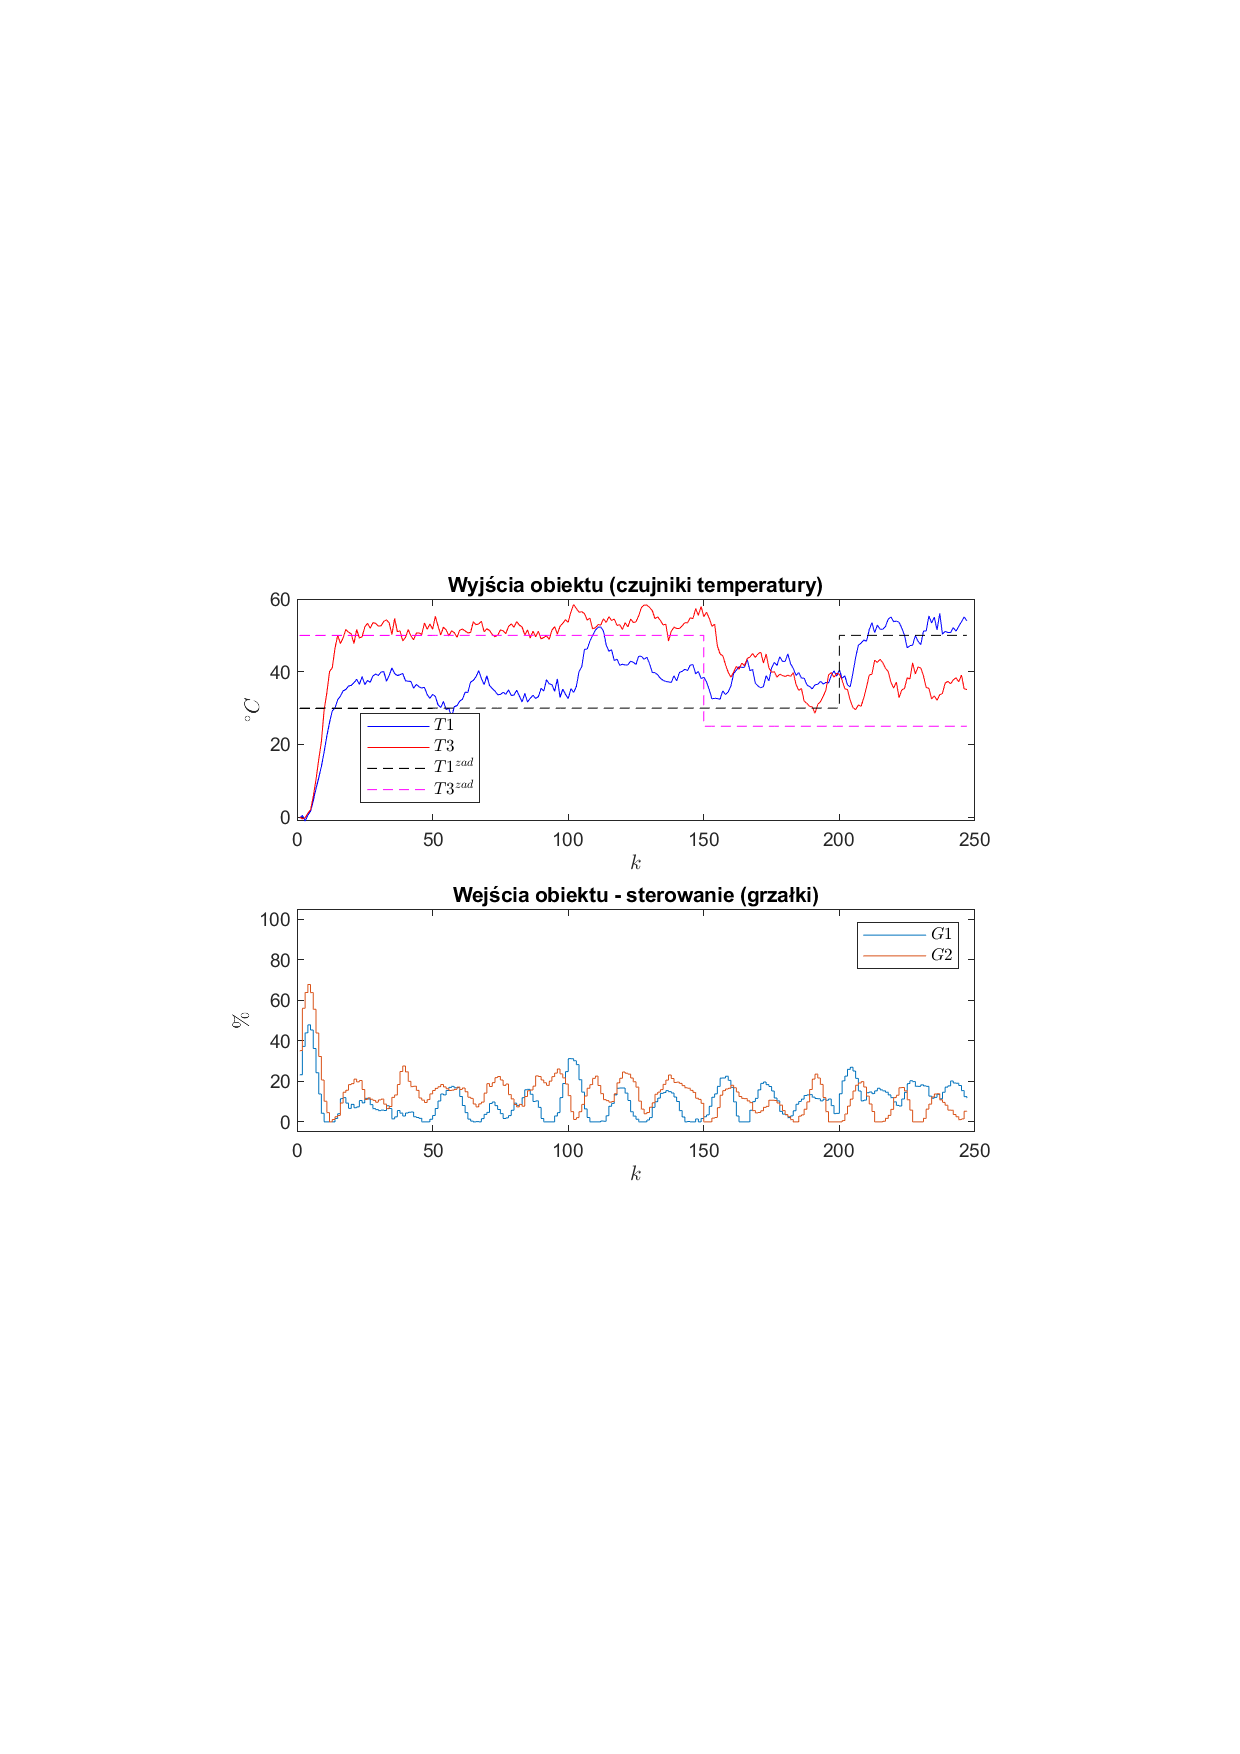
\includegraphics[scale=0.85, trim={2cm 8.5cm 2cm 8.5cm}]{rysunki/dmc_lambda1}
	\caption{Symulacja procesu dla $\lambda=1$}
	\label{dmc_lambda1}
\end{figure}


\begin{figure}
	\centering
	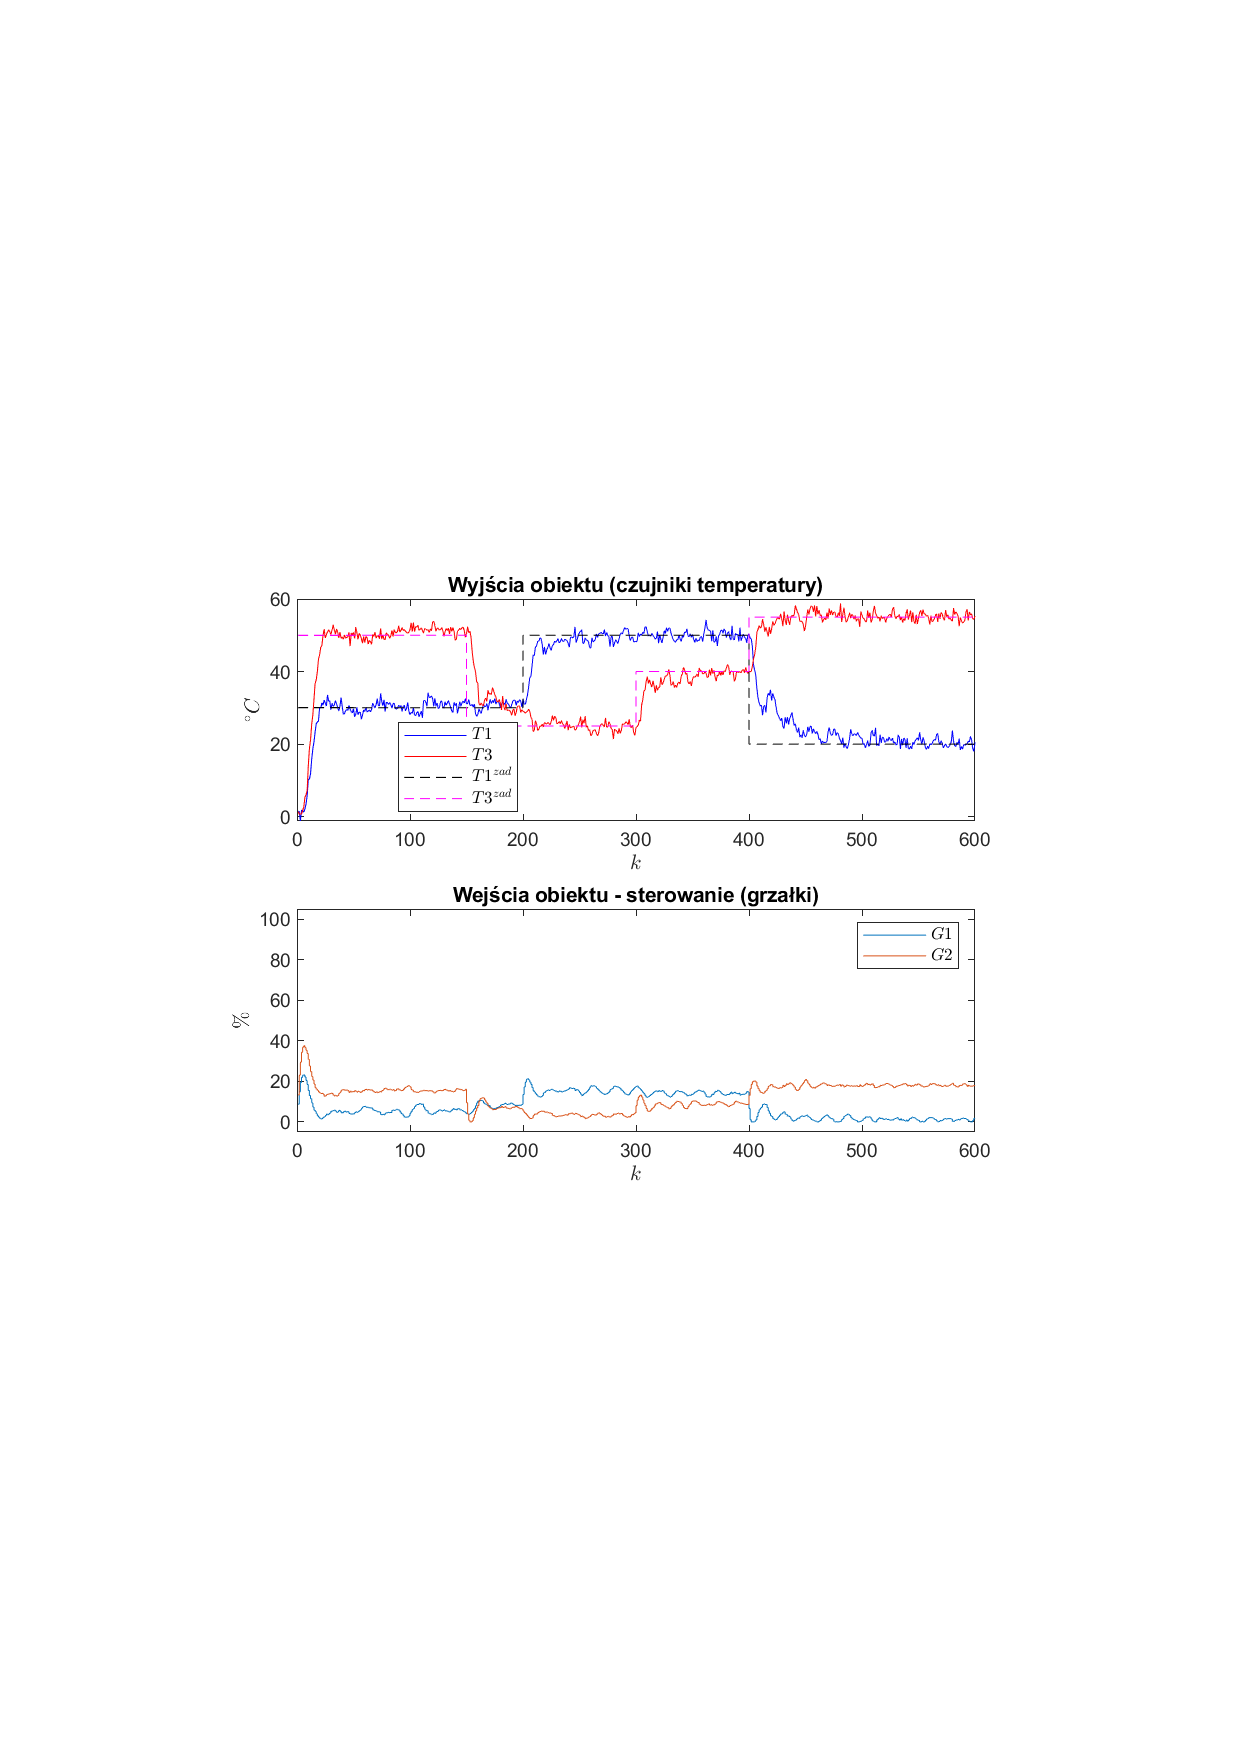
\includegraphics[scale=0.85, trim={2cm 8.5cm 2cm 8.5cm}]{rysunki/dmc_lambda10}
	\caption{Symulacja procesu dla $\lambda=10$}
	\label{dmc_lambda10}
\end{figure}

Ostatecznie przyj�li�my nast�puj�ce nastawy regulatora DMC

\begin{equation}
\label{dmc_final}
N=20, N_\mathrm{u}=3, \lambda=10
\end{equation}

Parametry te zapewni�y poprawn� prac� regulatora. 


\section{Implementacja}
Do kalibracji oraz symulacji algorytmu DMC wykorzystali�my skrypt \verb+DMC_MIMO.m+

\end{document}

